


\section{Results}



\subsection{Previous Results}

As mentioned previously, this project is a continuation of a project done over the previous year in
which we developed a method to use pulsar timing data to constrain our models. The final results of
that project were a set of models that accurately reproduce all observables and fully incorporated
the pulsar data. Figure \ref{fig:nobin_obs_panel} shows the model fits to most of the observables
while Figure \ref{fig:nobin_mass_fun} shows the fit to the stellar mass function data. In both
cases, the models satisfyingly reproduce all observables. The median and $1\sigma$ intervals of the
best fit parameters are listed in Table \ref{tab:parameters_nobin}.

One of the most interesting results of the previous project was the models' ability to constrain the
black hole content within 47\,Tuc. Figure \ref{fig:prev_nobin_BH_dists} shows the distribution of
mass in black hole mass and number of black holes in our set of best fit models, which come out to
$242^{+245}_{-148} \mathrm{M}_\odot$ and $41^{+27}_{-22}$ respectively. Both the total mass and
number are quite well contained especially in comparison to the previous constraints in the
literature \citep[see e.g.][]{Henault-Brunet2020,Weatherford2019}.




\begin{table}
	\centering
	\caption{Best fit parameters with $1\sigma$ intervals for models with a binary fraction of $0\%$.}
	\begin{tabular}{l l}

		\hline
		Parameter                 & Value                  \\
		\hline
		$\Phi_0$                  & $6.62^{+0.11}_{-0.11}$ \\
		$M/10^6 \mathrm{M}_\odot$ & $0.88^{+0.01}_{-0.01}$ \\
		$r_h / pc$                & $6.82^{+0.08}_{-0.07}$ \\
		$\log{r_a / pc}$          & $1.33^{+0.04}_{-0.04}$ \\
		$g$                       & $1.03^{+0.08}_{-0.08}$ \\
		$\delta$                  & $0.37^{+0.02}_{-0.01}$ \\
		$s^2$                     & $0.01^{+0.03}_{-0.01}$ \\
		$F$                       & $3.49^{+0.25}_{-0.22}$ \\
		$\alpha_1$                & $0.47^{+0.06}_{-0.05}$ \\
		$\alpha_2$                & $1.18^{+0.06}_{-0.07}$ \\
		$\alpha_3$                & $2.15^{+0.04}_{-0.04}$ \\
		$BH_{ret} (\%)$           & $0.13^{+0.13}_{-0.08}$ \\
		$d$                       & $4.42^{+0.02}_{-0.02}$ \\
		\hline
	\end{tabular}
	\label{tab:parameters_nobin}
\end{table}

\begin{figure}
	\centering
	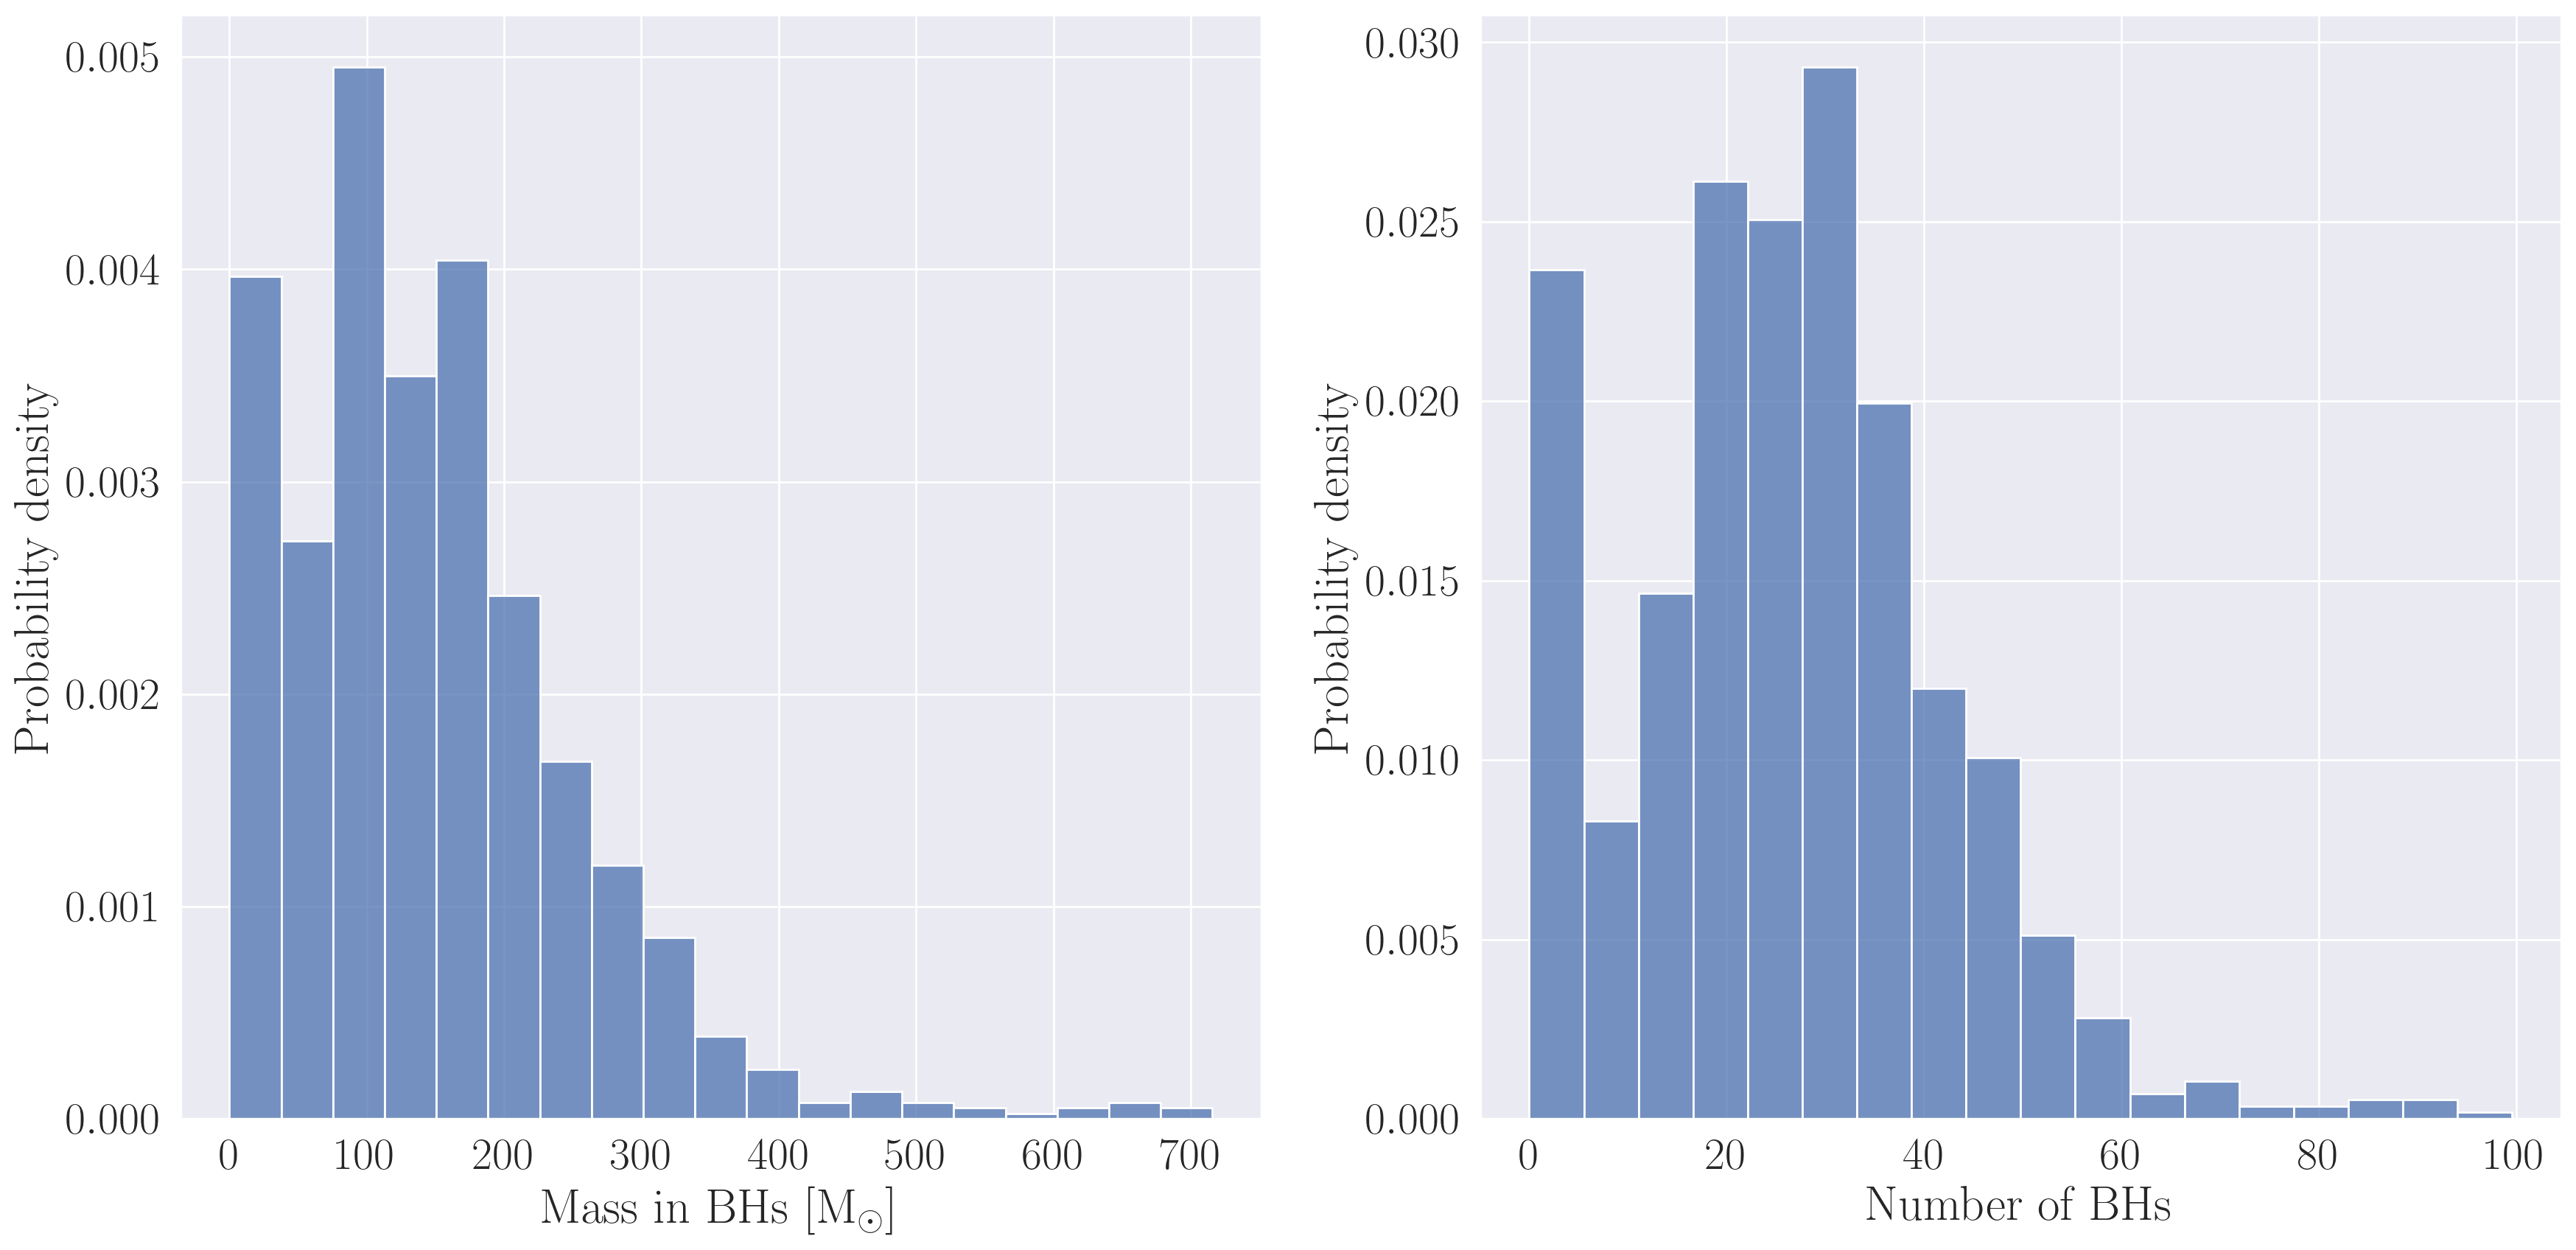
\includegraphics[width=0.8\textwidth]{figures/prev_nobin/BH_dists.png}
	\caption{BH distributions}
	\label{fig:prev_nobin_BH_dists}
\end{figure}


\subsection{Low Binary Fraction}

In the models with a $2\%$ binary fraction, we find a similar ability to reproduce all the
observables, Figure \ref{fig:low_bin_model_obs_panel} and Figure \ref{fig:low_bin_model_mass_fun}
show the model fits compared to the data. Once again the models satisfyingly reproduce all
observables.

The black hole content in these models is also quite well contained, though different from the
models without binaries. Figure \ref{fig:low_bin_model_BH_dists} shows the distribution of mass in
black holes and number of black holes which this time, work out to $22^{+13}_{-19}$ black holes or
$114^{+79}_{-144} \mathrm{M}_\odot$ in black holes. The best-fit parameters and the $1\sigma$
intervals for this set of models are listed in Table \ref{tab:parameters_lowbin}.


\begin{table}
	\centering
	\caption{Best fit parameters with $1\sigma$ intervals for models with a $2\%$ binary fraction.}
	\begin{tabular}{l l}

		\hline
		Parameter                 & Value                  \\
		\hline
		$\Phi_0$                  & $6.28^{+0.10}_{-0.10}$ \\
		$M/10^6 \mathrm{M}_\odot$ & $0.89^{+0.01}_{-0.01}$ \\
		$r_h / pc$                & $6.74^{+0.06}_{-0.06}$ \\
		$\log{r_a / pc}$          & $1.50^{+0.06}_{-0.05}$ \\
		$g$                       & $1.36^{+0.06}_{-0.06}$ \\
		$\delta$                  & $0.43^{+0.02}_{-0.02}$ \\
		$s^2$                     & $0.01^{+0.01}_{-0.00}$ \\
		$F$                       & $3.24^{+0.13}_{-0.12}$ \\
		$\alpha_1$                & $0.37^{+0.02}_{-0.02}$ \\
		$\alpha_2$                & $1.47^{+0.05}_{-0.05}$ \\
		$\alpha_3$                & $2.18^{+0.04}_{-0.04}$ \\
		$BH_{ret} (\%)$           & $0.08^{+0.09}_{-0.05}$ \\
		$d$                       & $4.42^{+0.02}_{-0.02}$ \\
		\hline
	\end{tabular}
	\label{tab:parameters_lowbin}
\end{table}

\begin{figure}
	\centering
	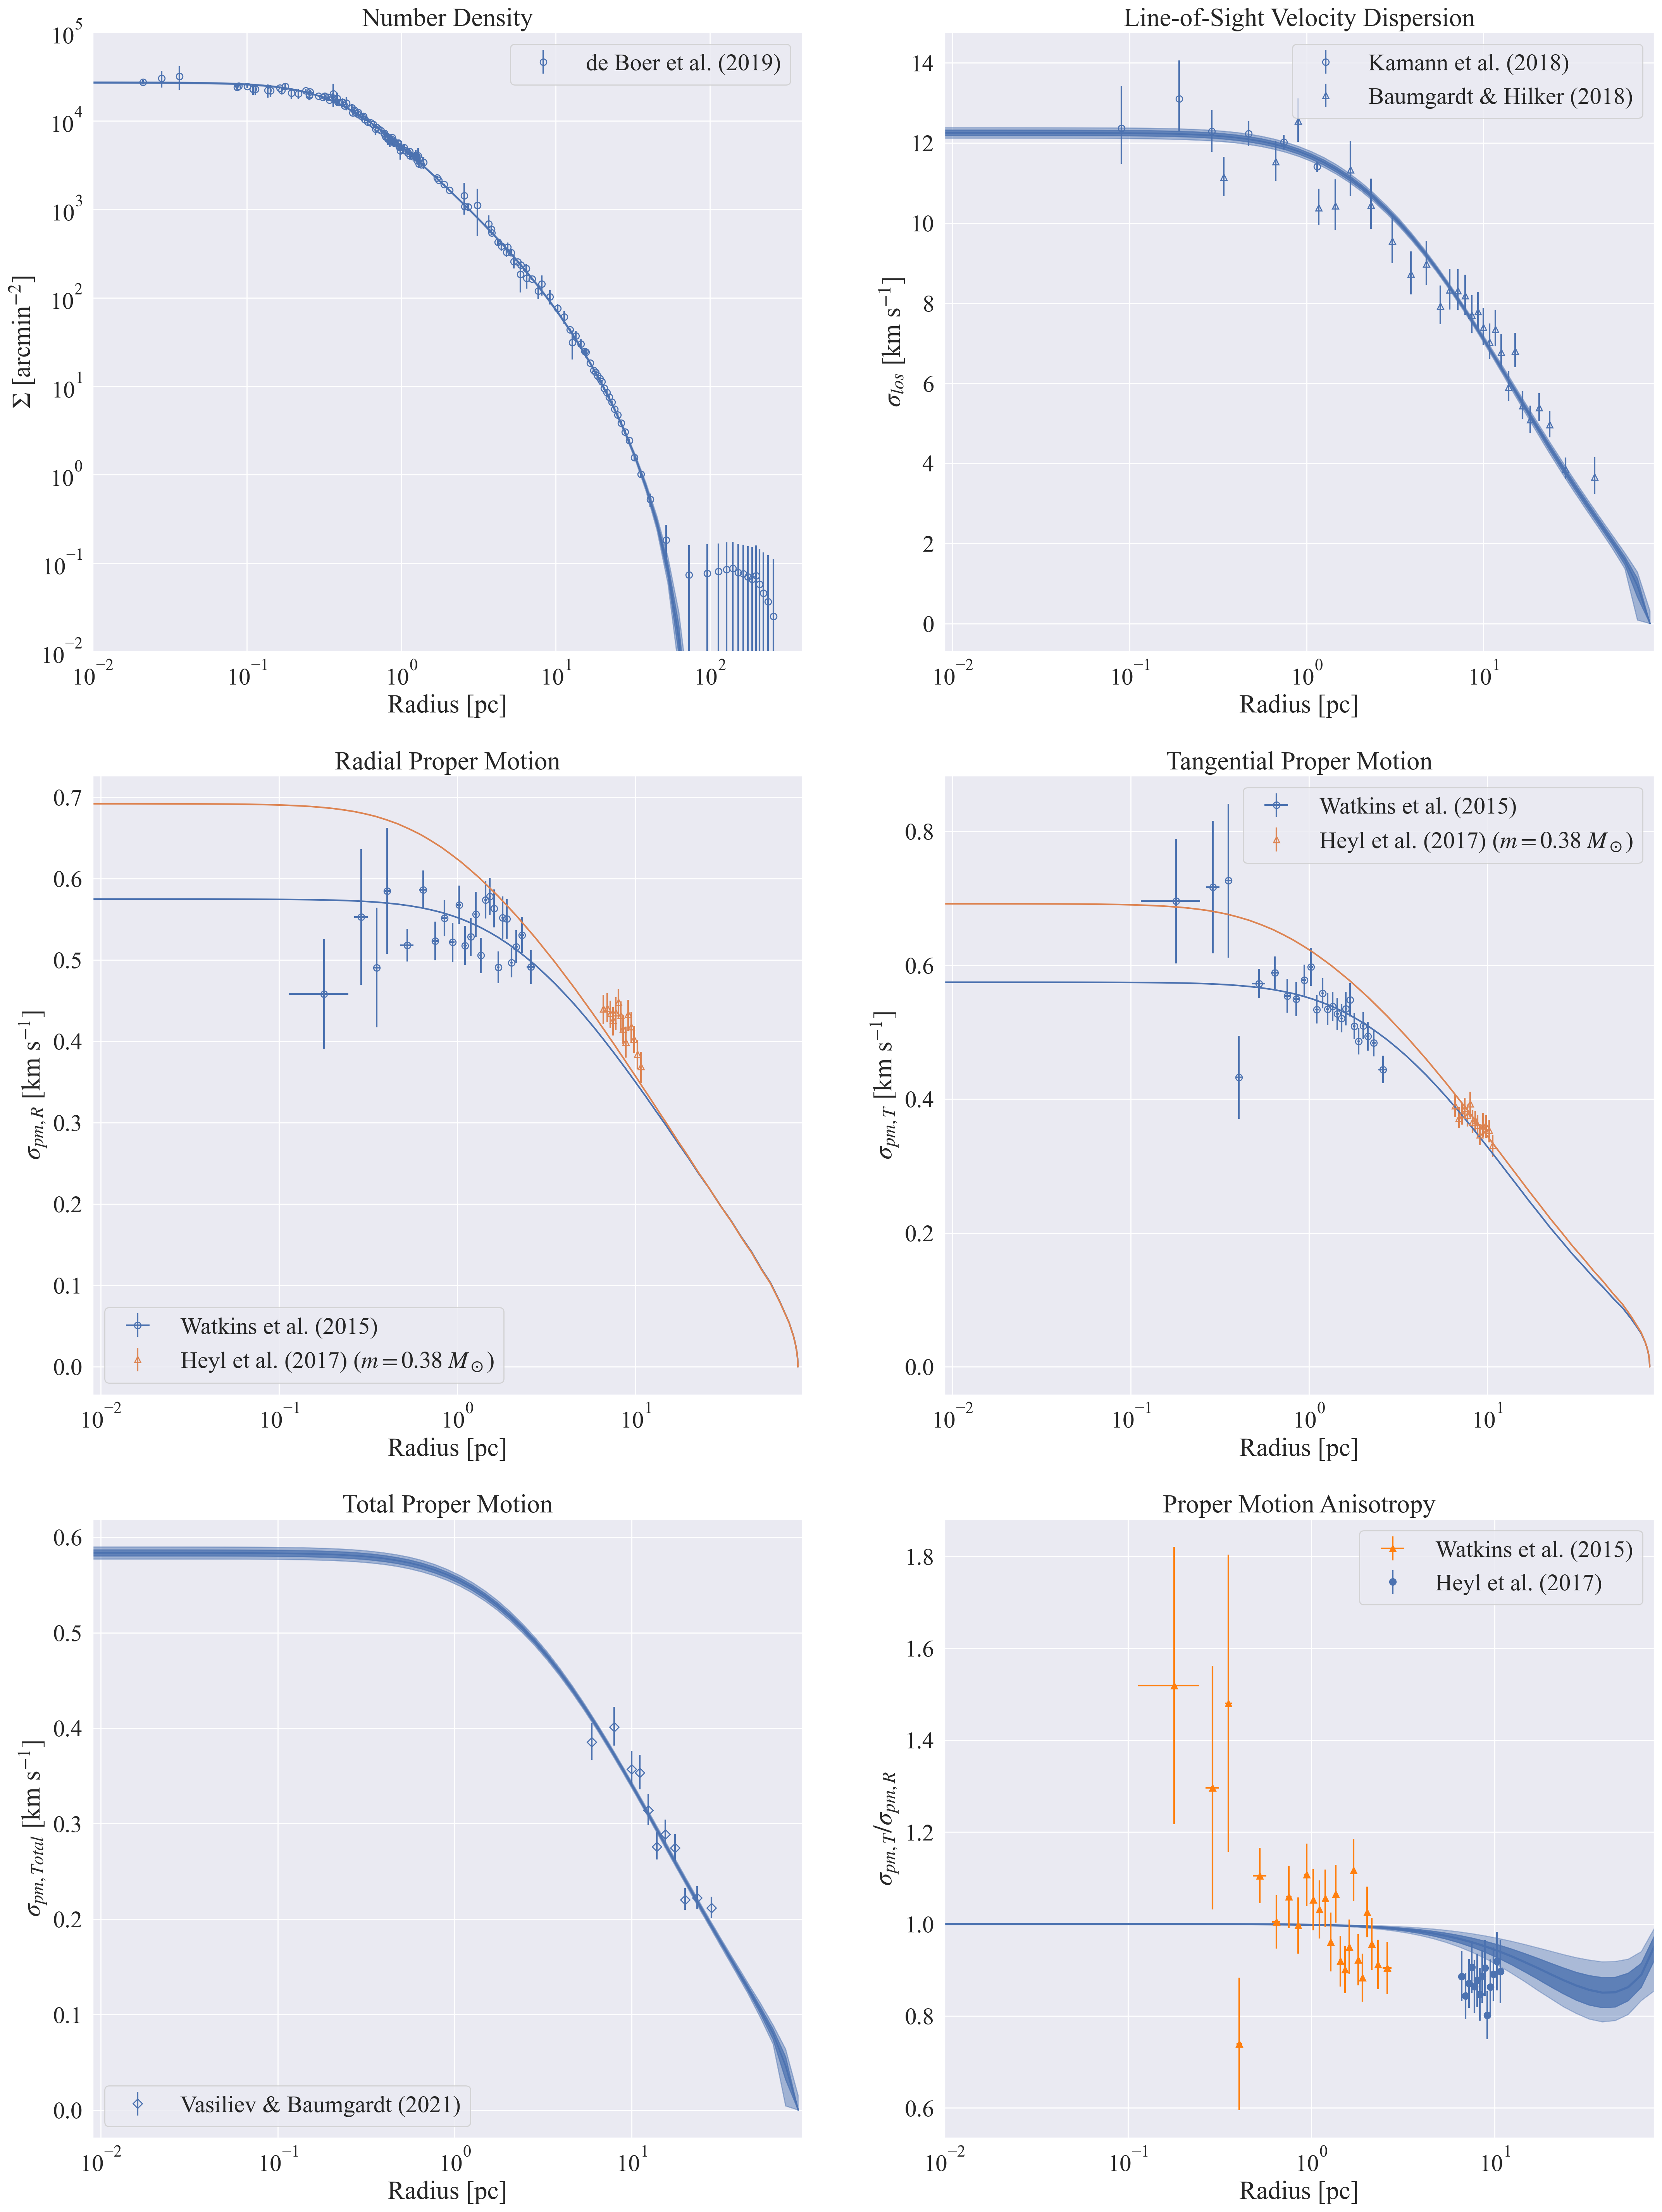
\includegraphics[width=0.9\textwidth]{figures/low_bin_model/obs_panel.png}
	\caption{Model fits to observable for models with a $2\%$ binary fraction.}
	\label{fig:low_bin_model_obs_panel}
\end{figure}


\begin{figure}
	\centering
	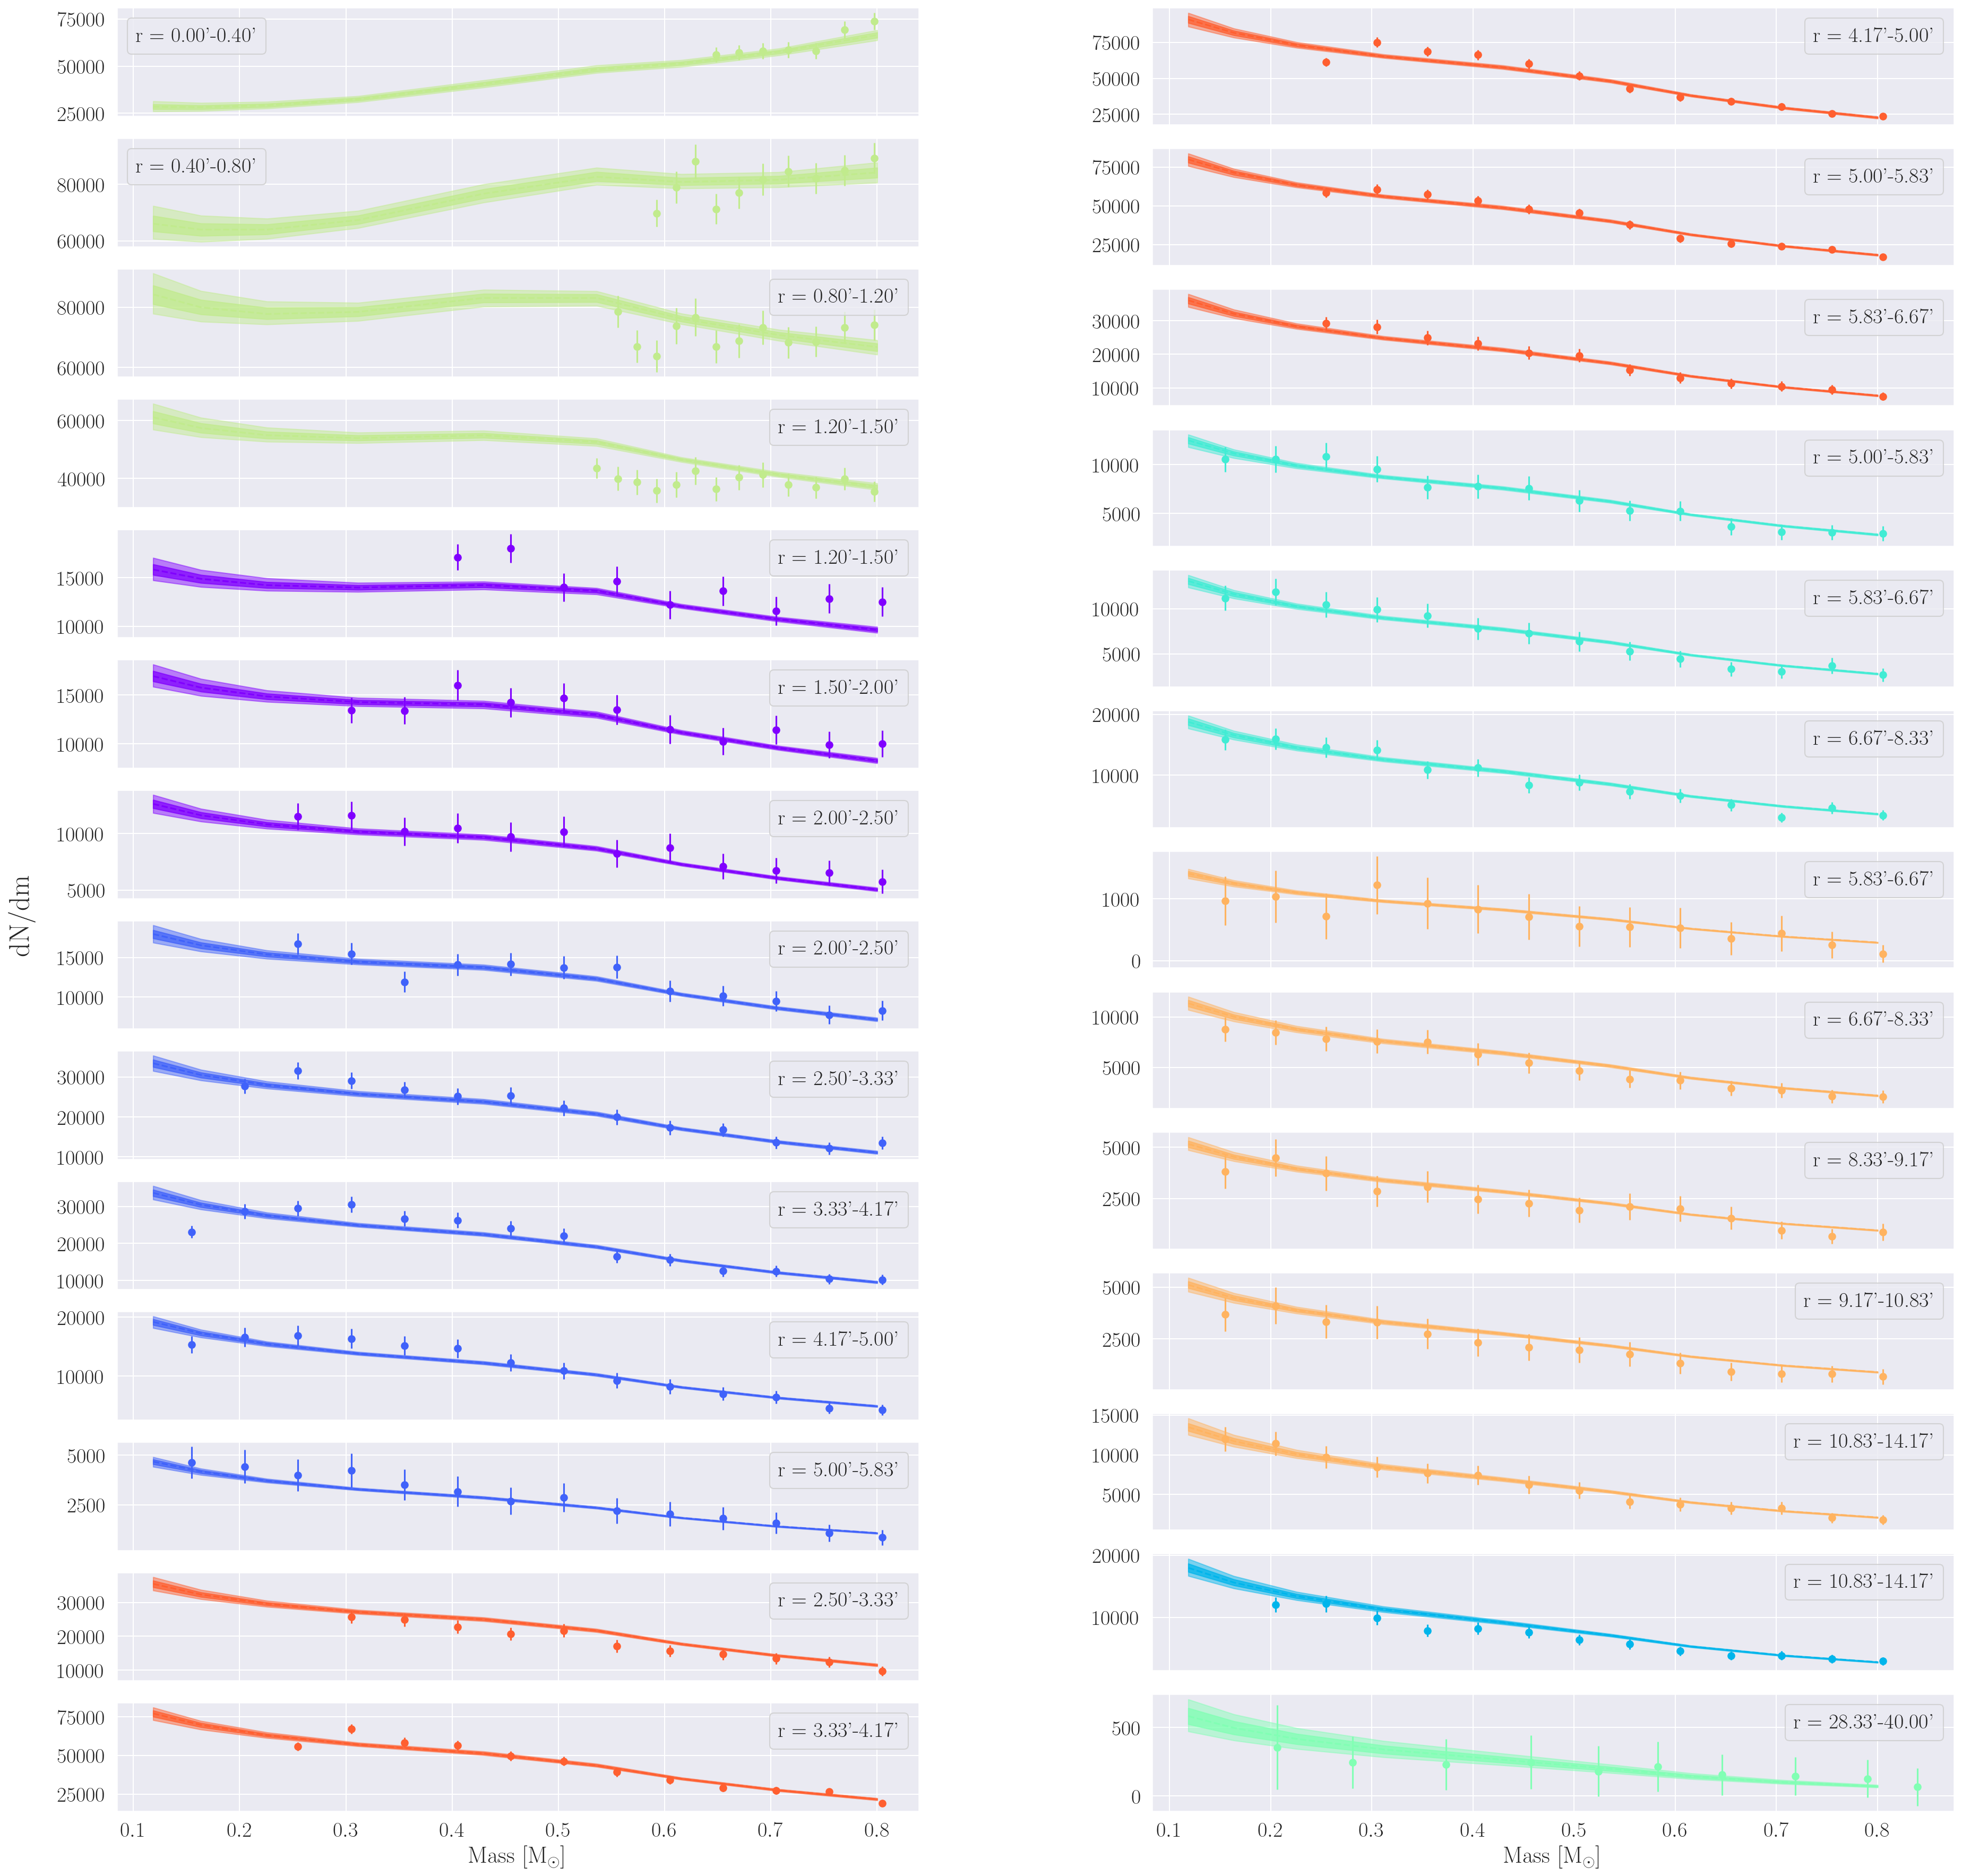
\includegraphics[width=\textwidth]{figures/low_bin_model/mass_fun.png}
	\caption{Model fits to stellar mass function data for models with a $2\%$ binary fraction.}
	\label{fig:low_bin_model_mass_fun}
\end{figure}



\begin{figure}
	\centering
	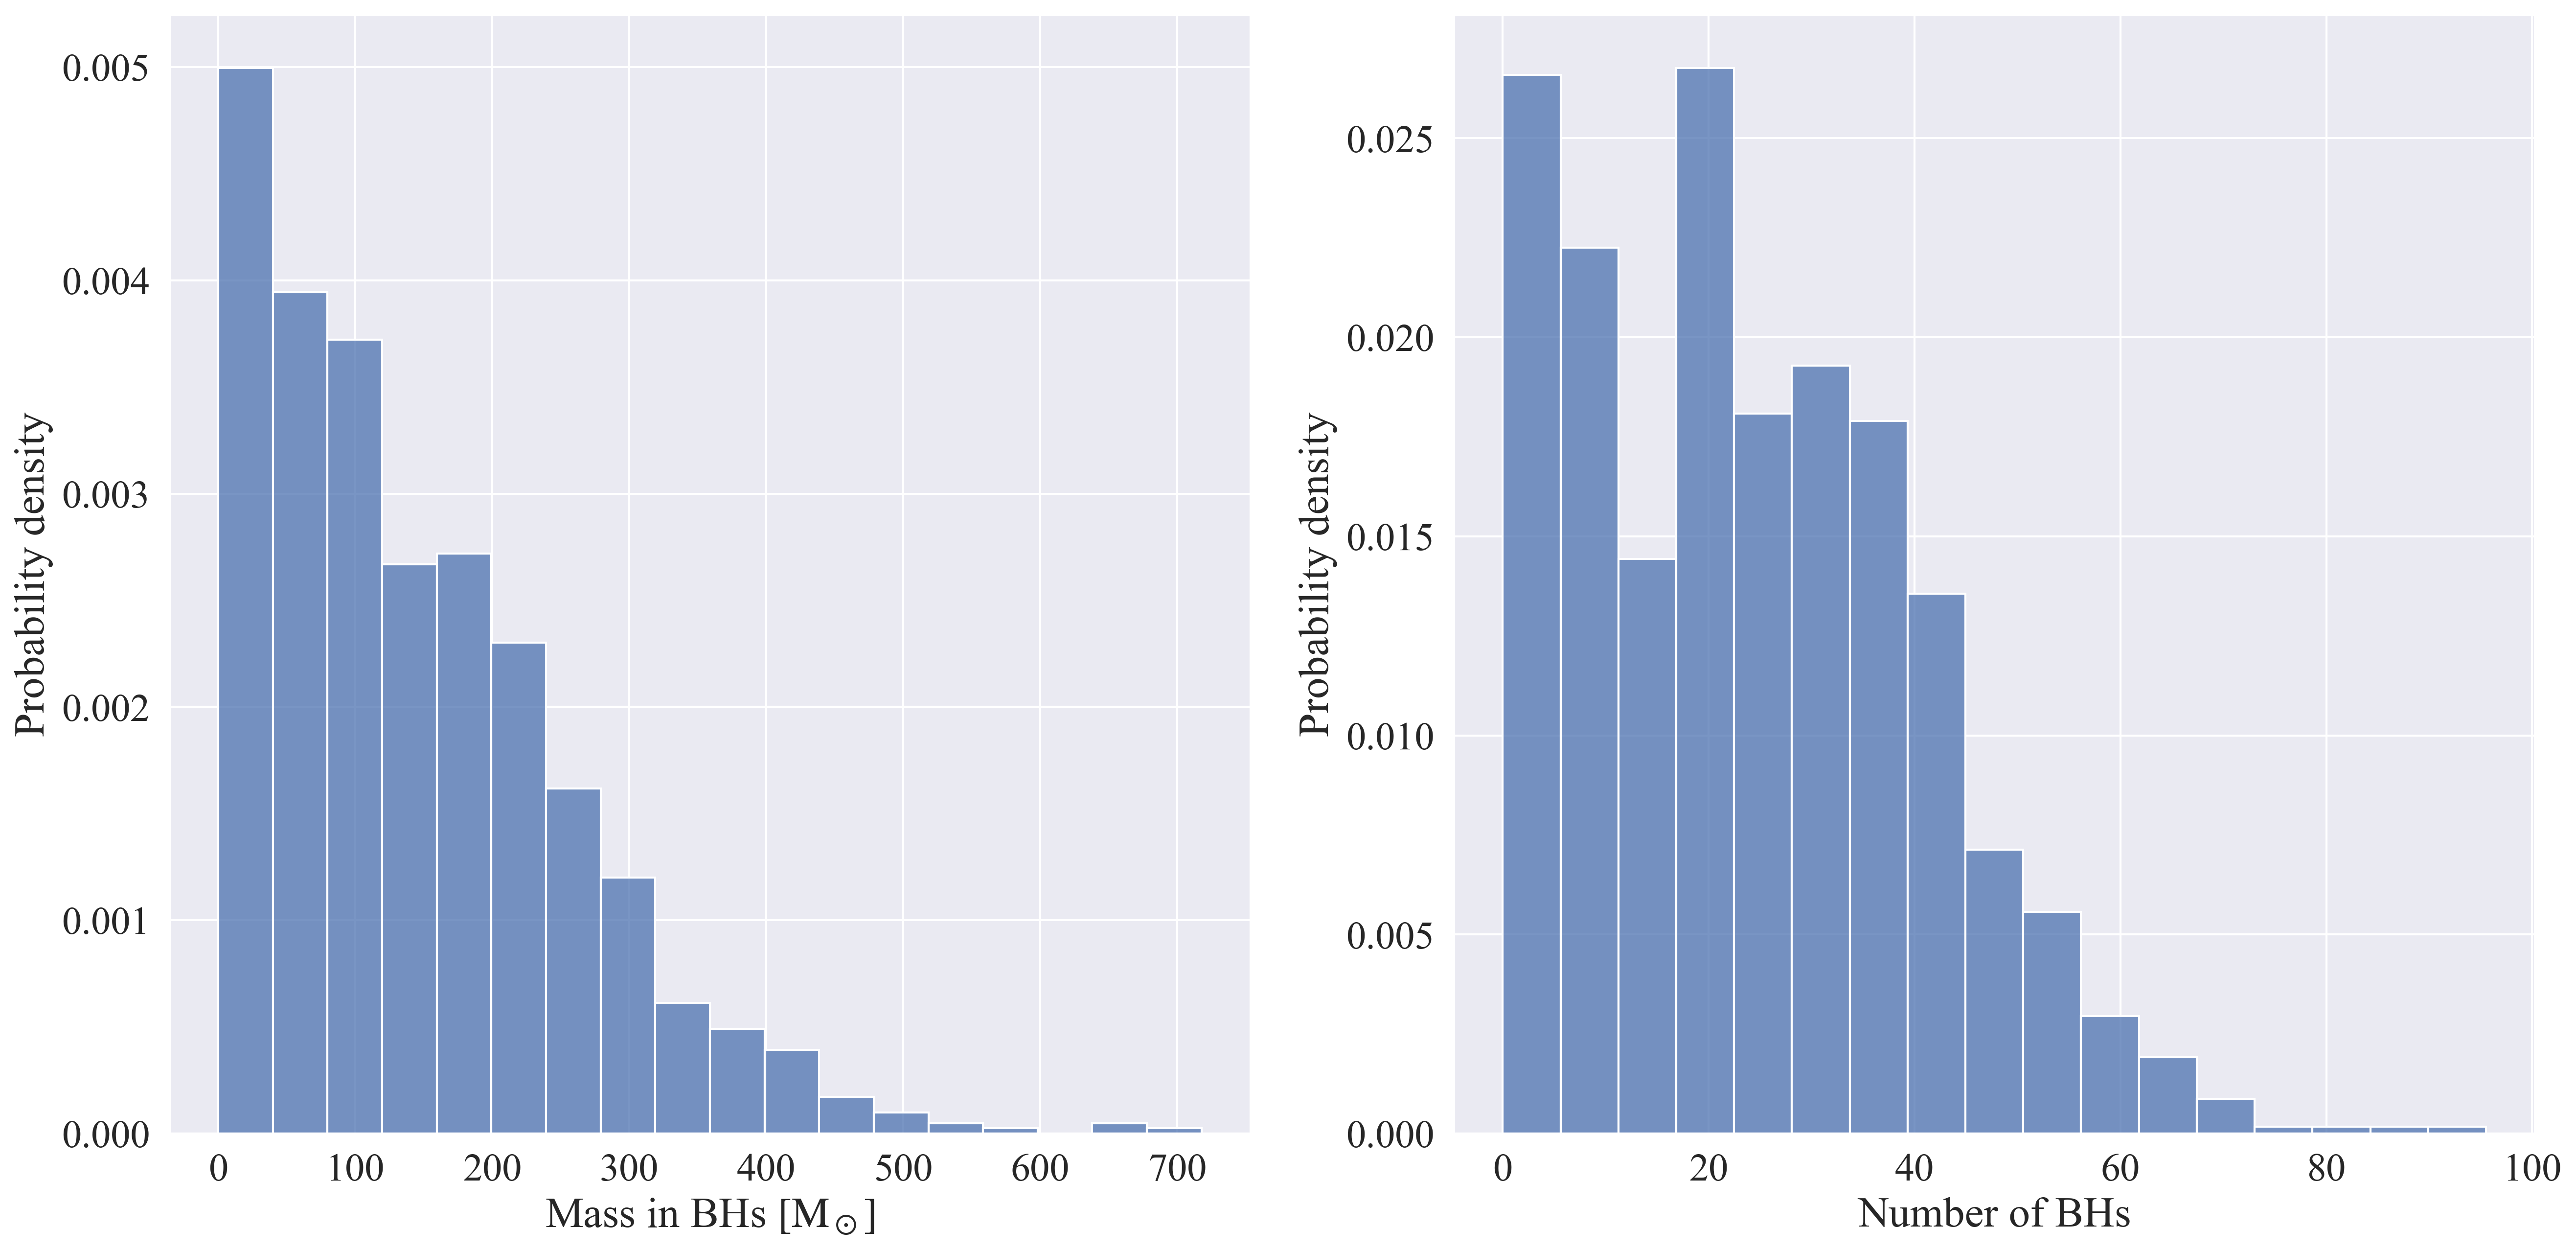
\includegraphics[width=0.8\textwidth]{figures/low_bin_model/BH_dists.png}
	\caption{Distribution in mass and number of black holes for models with a $2\%$ binary fraction.}
	\label{fig:low_bin_model_BH_dists}
\end{figure}


A binary fraction of $2\%$ results in a total mass in binaries of around $15800 \mathrm{M}_\odot$,
Figure \ref{fig:low_bin_model_Bin_mass} shows the distribution of mass in binaries in our set of
best-fitting models.


\begin{figure}
	\centering
	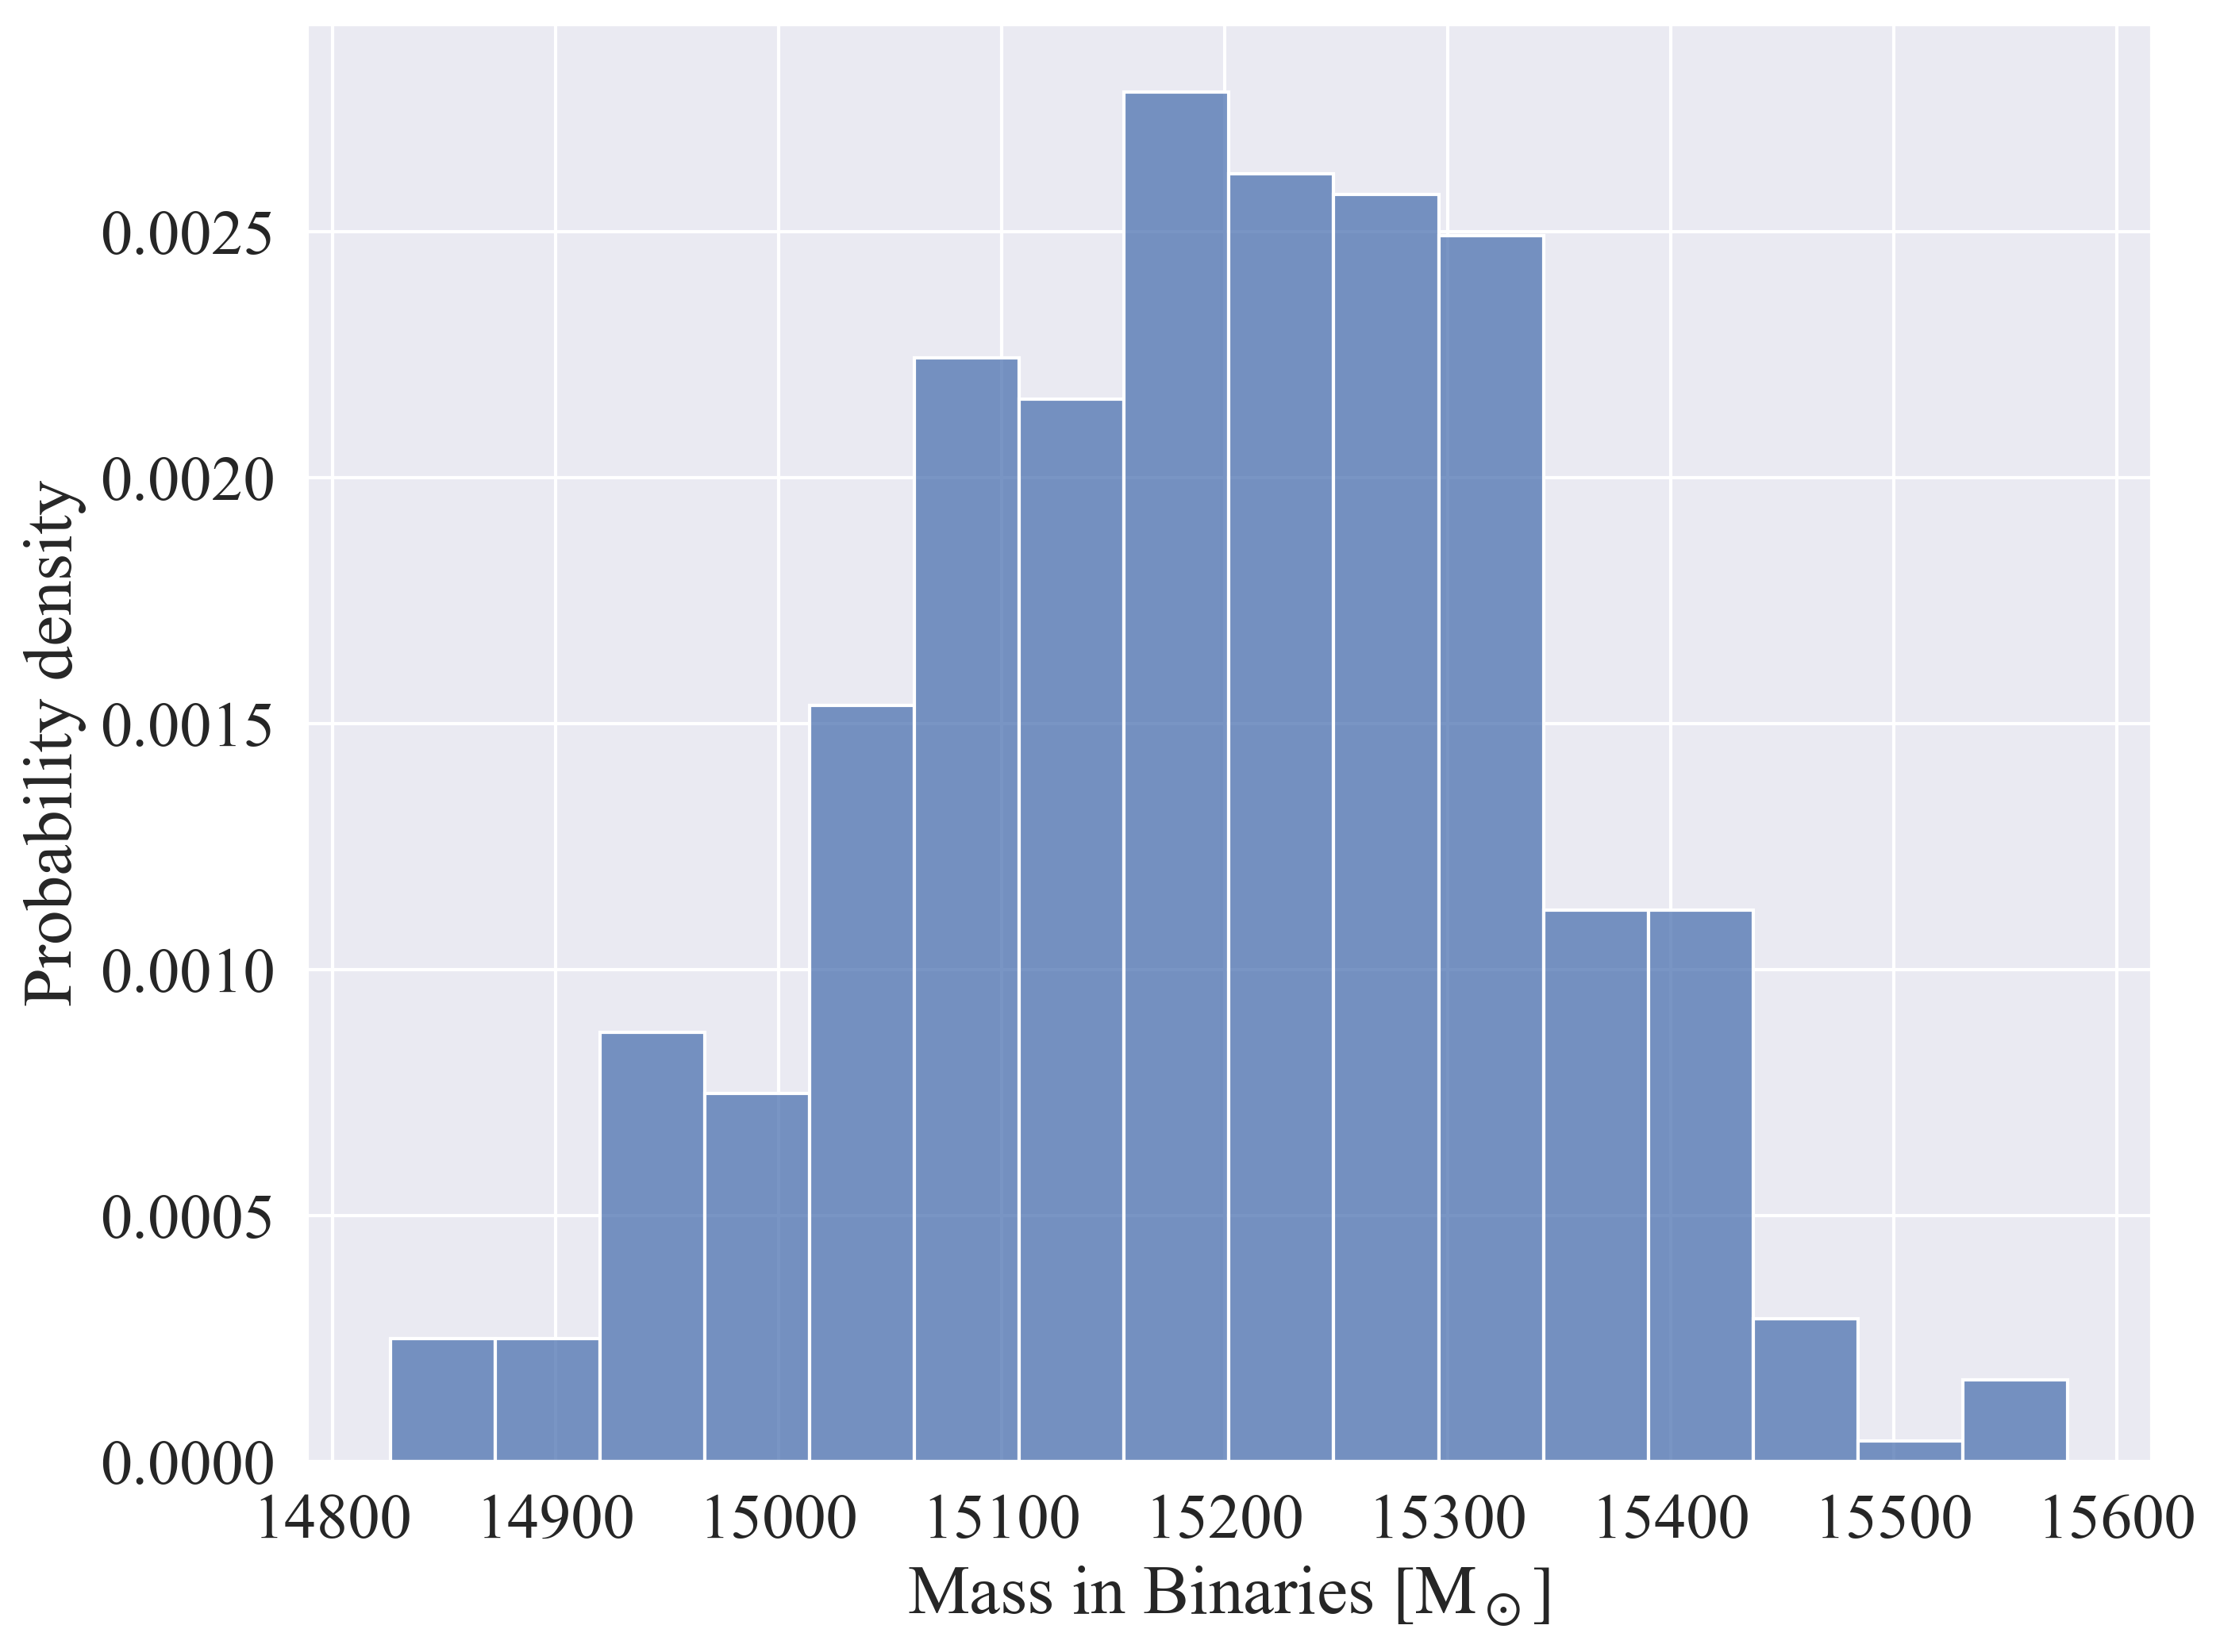
\includegraphics[width=0.8\textwidth]{figures/low_bin_model/binary_mass.png}
	\caption{Distribution of mass in binaries for models with a $2\%$ binary fraction.}
	\label{fig:low_bin_model_Bin_mass}
\end{figure}


\subsection{High Binary Fraction}

As is the case for the models with a low binary fraction, the models with a $10\%$ binary
fraction fit the observables very well. Figures \ref{fig:highbin_obs_panel} and
\ref{fig:highbin_mass_fun} show the model fits compared to the data.

\begin{table}
	\centering
	\caption{Best fit parameters with $1\sigma$ intervals for models with a $10\%$ binary fraction.}
	\begin{tabular}{l l}

		\hline
		Parameter                 & Value                  \\
		\hline
		$\Phi_0$                  & $6.36^{+0.09}_{-0.09}$ \\
		$M/10^6 \mathrm{M}_\odot$ & $0.89^{+0.01}_{-0.01}$ \\
		$r_h / pc$                & $6.77^{+0.06}_{-0.06}$ \\
		$\log{r_a / pc}$          & $1.48^{+0.06}_{-0.05}$ \\
		$g$                       & $1.34^{+0.06}_{-0.06}$ \\
		$\delta$                  & $0.41^{+0.01}_{-0.01}$ \\
		$s^2$                     & $0.01^{+0.01}_{-0.00}$ \\
		$F$                       & $3.16^{+0.13}_{-0.12}$ \\
		$\alpha_1$                & $0.45^{+0.02}_{-0.02}$ \\
		$\alpha_2$                & $1.53^{+0.05}_{-0.04}$ \\
		$\alpha_3$                & $2.46^{+0.05}_{-0.05}$ \\
		$BH_{ret} (\%)$           & $0.17^{+0.18}_{-0.12}$ \\
		$d$                       & $4.43^{+0.02}_{-0.02}$ \\
		\hline
	\end{tabular}
	\label{tab:parameters_highbin}
\end{table}

With a higher binary fraction, we now find fewer black holes, Figure
\ref{fig:high_bin_model_BH_dists} shows the distribution in mass and number which come out to
$12^{+13}_{-12}$ black holes or $81 ^{+121}_{-81} \mathrm{M}_\odot$ in black holes.


\begin{figure}
	\centering
	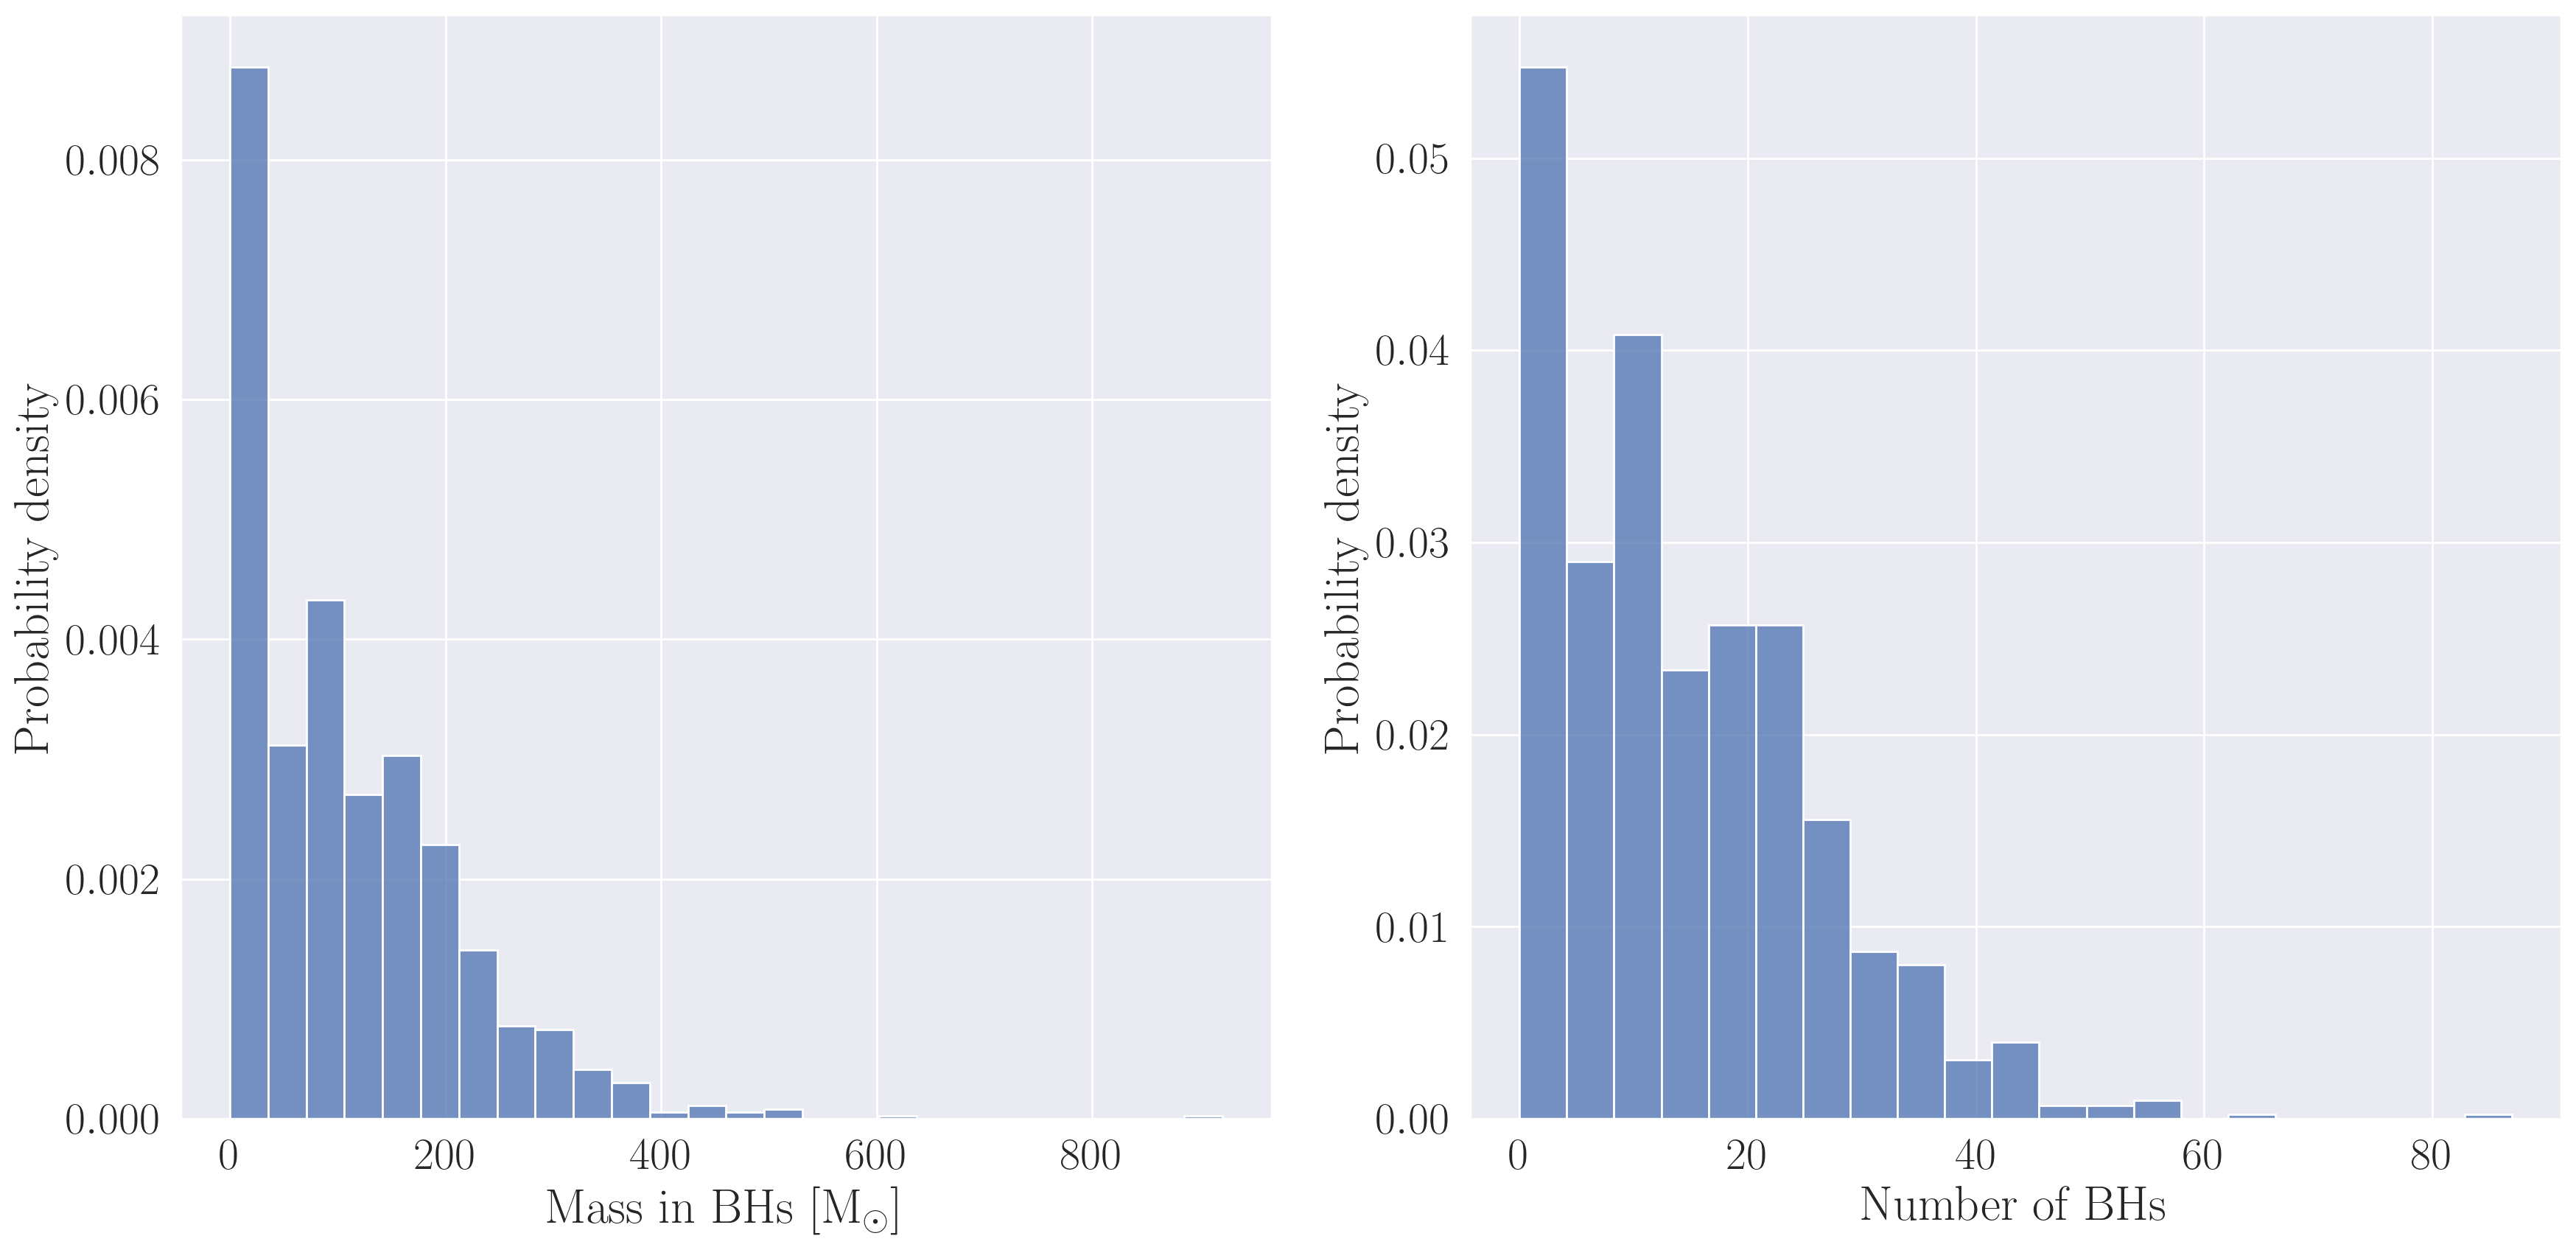
\includegraphics[width=0.8\textwidth]{figures/high_bin_model/BH_dists.png}
	\caption{Distribution in mass and number for models with a $10\%$ binary fraction.}
	\label{fig:high_bin_model_BH_dists}
\end{figure}


With a $10\%$ binary fraction we now have a significant amount of mass in binaries, roughly $15800
	\mathrm{M_\odot}$ (see figure \ref{fig:high_bin_model_Bin_mass}), which is a bit less than $2\%$ of
the total cluster mass.

\begin{figure}
	\centering
	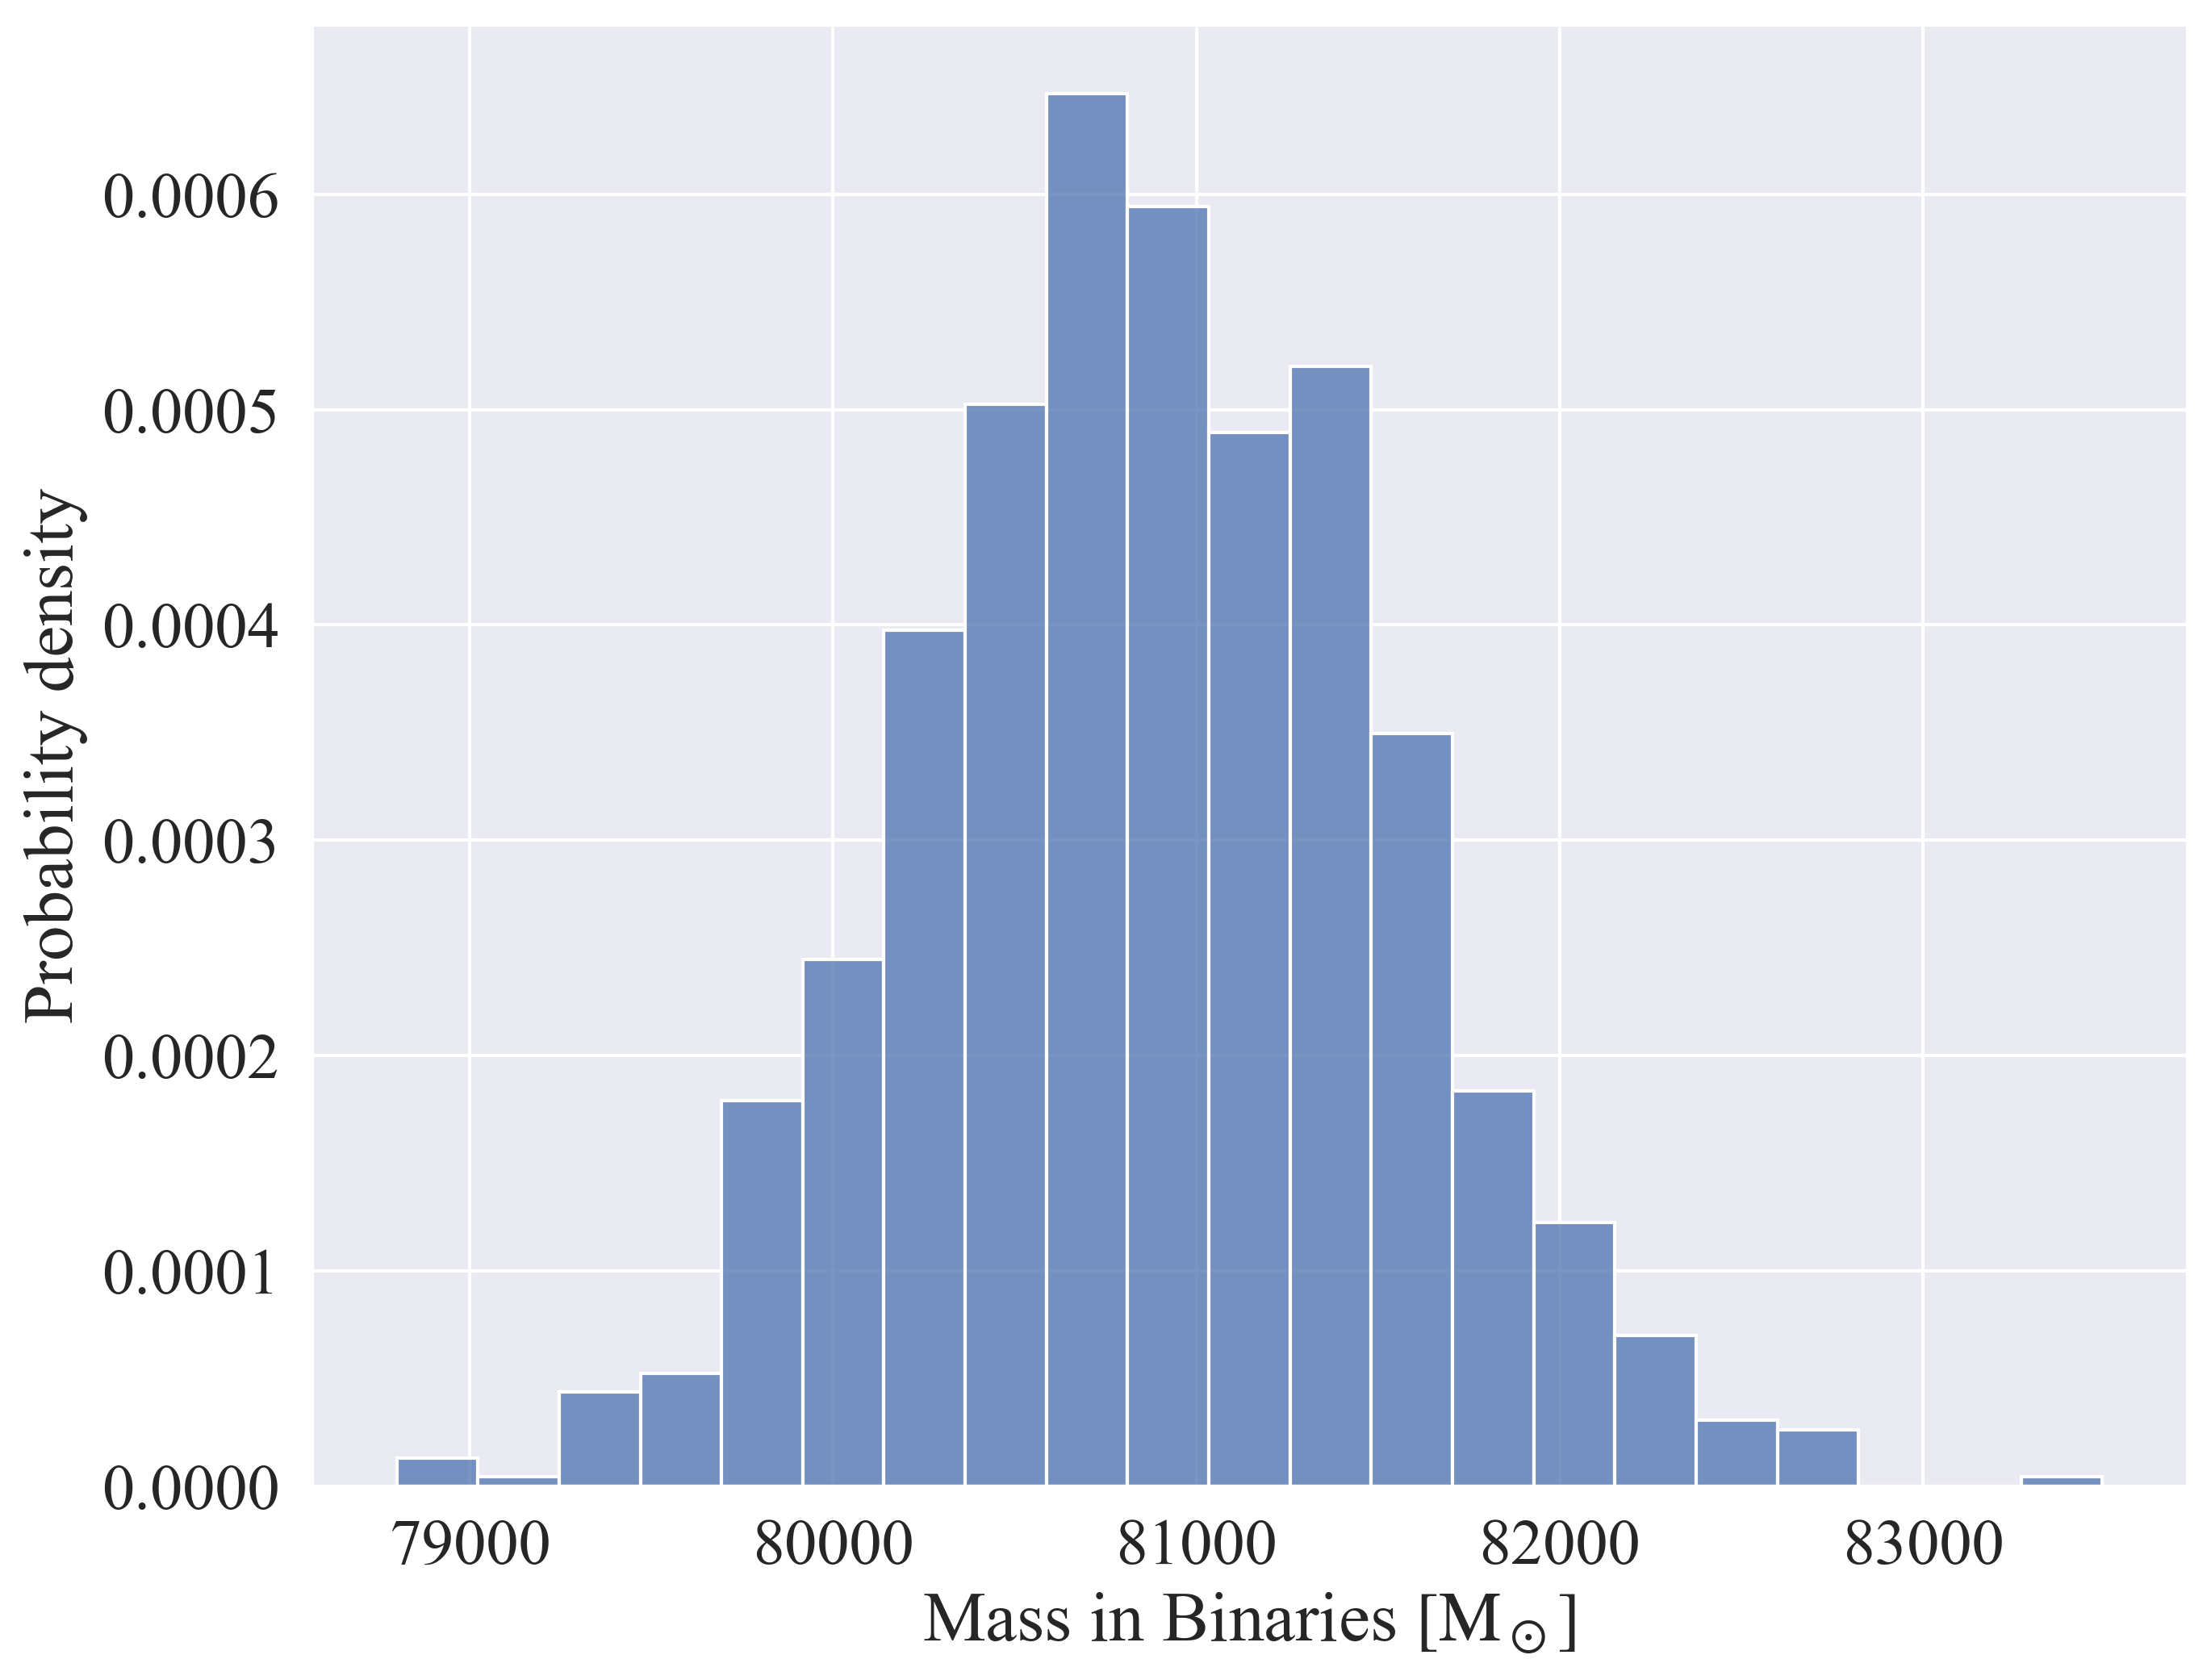
\includegraphics[width=0.8\textwidth]{figures/high_bin_model/binary_mass.png}
	\caption{Distribution of mass in binaries for models with a $10\%$ binary fraction.}
	\label{fig:high_bin_model_Bin_mass}
\end{figure}





\section{Discussion}








\begin{table}
	\centering
	\caption{Best fit parameters with $1\sigma$ intervals for all sets of models.}
	\begin{tabular}{l l l l}

		\hline
		Parameter                 & Value                                                                    \\
		\hline
		$f_b$                     & $0\%$                  & $2\%$                  & $10\%$                 \\
		$\Phi_0$                  & $6.62^{+0.11}_{-0.11}$ & $6.28^{+0.10}_{-0.10}$ & $6.36^{+0.09}_{-0.09}$ \\
		$M/10^6 \mathrm{M}_\odot$ & $0.88^{+0.01}_{-0.01}$ & $0.89^{+0.01}_{-0.01}$ & $0.89^{+0.01}_{-0.01}$ \\
		$r_h / pc$                & $6.82^{+0.08}_{-0.07}$ & $6.74^{+0.06}_{-0.06}$ & $6.77^{+0.06}_{-0.06}$ \\
		$\log{r_a / pc}$          & $1.33^{+0.04}_{-0.04}$ & $1.50^{+0.06}_{-0.05}$ & $1.48^{+0.06}_{-0.05}$ \\
		$g$                       & $1.03^{+0.08}_{-0.08}$ & $1.36^{+0.06}_{-0.06}$ & $1.34^{+0.06}_{-0.06}$ \\
		$\delta$                  & $0.37^{+0.02}_{-0.01}$ & $0.43^{+0.02}_{-0.02}$ & $0.41^{+0.01}_{-0.01}$ \\
		$s^2$                     & $0.01^{+0.03}_{-0.01}$ & $0.01^{+0.01}_{-0.00}$ & $0.01^{+0.01}_{-0.00}$ \\
		$F$                       & $3.49^{+0.25}_{-0.22}$ & $3.24^{+0.13}_{-0.12}$ & $3.16^{+0.13}_{-0.12}$ \\
		$\alpha_1$                & $0.47^{+0.06}_{-0.05}$ & $0.37^{+0.02}_{-0.02}$ & $0.45^{+0.02}_{-0.02}$ \\
		$\alpha_2$                & $1.18^{+0.06}_{-0.07}$ & $1.47^{+0.05}_{-0.05}$ & $1.53^{+0.05}_{-0.04}$ \\
		$\alpha_3$                & $2.15^{+0.04}_{-0.04}$ & $2.18^{+0.04}_{-0.04}$ & $2.46^{+0.05}_{-0.05}$ \\
		$BH_{ret} (\%)$           & $0.13^{+0.13}_{-0.08}$ & $0.08^{+0.09}_{-0.05}$ & $0.17^{+0.18}_{-0.12}$ \\
		$d$                       & $4.42^{+0.02}_{-0.02}$ & $4.42^{+0.02}_{-0.02}$ & $4.43^{+0.02}_{-0.02}$ \\
		\hline
	\end{tabular}
	\label{tab:parameters_all}
\end{table}







In each set of models, all observables are very well reproduced, showing the flexibility of the
\code{LIMEPY} models. Due to this flexibility, it is unlikely that with current observations we
would be able to infer anything about the binary population of a cluster using this technique.
Instead, this method should be used in cases where there are existing estimates of the binary
population within a cluster in order to add a realistic binary component to \code{LIMEPY} models



\subsection{The Effects of the Binaries}


Table \ref{tab:parameters_all} shows the recovered parameters for each set of models, we can see a
clear agreement in the recovered values which affect the overall structure of the cluster. In
particular, the total cluster mass, half-mass radius, anisotropy radius, truncation parameter,
degree of mass segregation and distance are all either identical or within $1\sigma$ of each other
for all three sets of models.

\ps{I'm thinking this might be even more pronounced after we rerun the no binary case, the 0 binary
	case should come more in-line with the other two cases.}


The most striking change in model parameters are the values pertaining to the mass function, in
particular, the $\alpha_3$ parameter which controls the slope of the high-mass mass function. In the
case with a $10\%$ binary fraction, this parameter is much larger than in the other two cases
showing that the abundance of binary stars reduce the need for high mass stars and remnants.

We can see that there is still some need for BHs in some of the models as the $BH_{ret}$ parameter
is much larger in the model with many binaries, this means that even though the initial mass
function produces many fewer black holes, more of these black holes need to be retained throughout
the evolution of the cluster.

Table \ref{tab:BH_contents} and Figure \ref{fig:BH_KDEs} show the distribution of BHs for each set
of models. We can see a clear decrease in the black hole content as we add more binaries. This
effect was also found by \citet{Mann2019} (see also associated erratum \citealt{Mann2020}) when they
modelled the central kinematics of 47\,Tuc. This effect is due to the high-mass binary systems which
have mass-segregated to the central regions of the cluster contribution to the overall mass
distribution in a similar way to heavy stellar remnants. Through this process, fewer black holes are
needed to create the observed central velocity dispersion other kinematics.


% Table comparing bh content in each set of models
\begin{table}
	\centering
	\caption{Black hole content in each set of models}
	\begin{tabular}{c c c}
		\hline
		Binary Fraction $(\%)$ & Mass in BHs                          & Number of BHs    \\
		\hline
		0                      & $240^{+245}_{-146} \mathrm{M}_\odot$ & $41^{+27}_{-22}$ \\
		2                      & $114^{+144}_{-79} \mathrm{M}_\odot$  & $22^{+19}_{-13}$ \\
		10                     & $81 ^{+121}_{-81} \mathrm{M}_\odot$  & $12^{+13}_{-12}$ \\
		\hline
	\end{tabular}
	\label{tab:BH_contents}
\end{table}


\begin{figure}
	\centering
	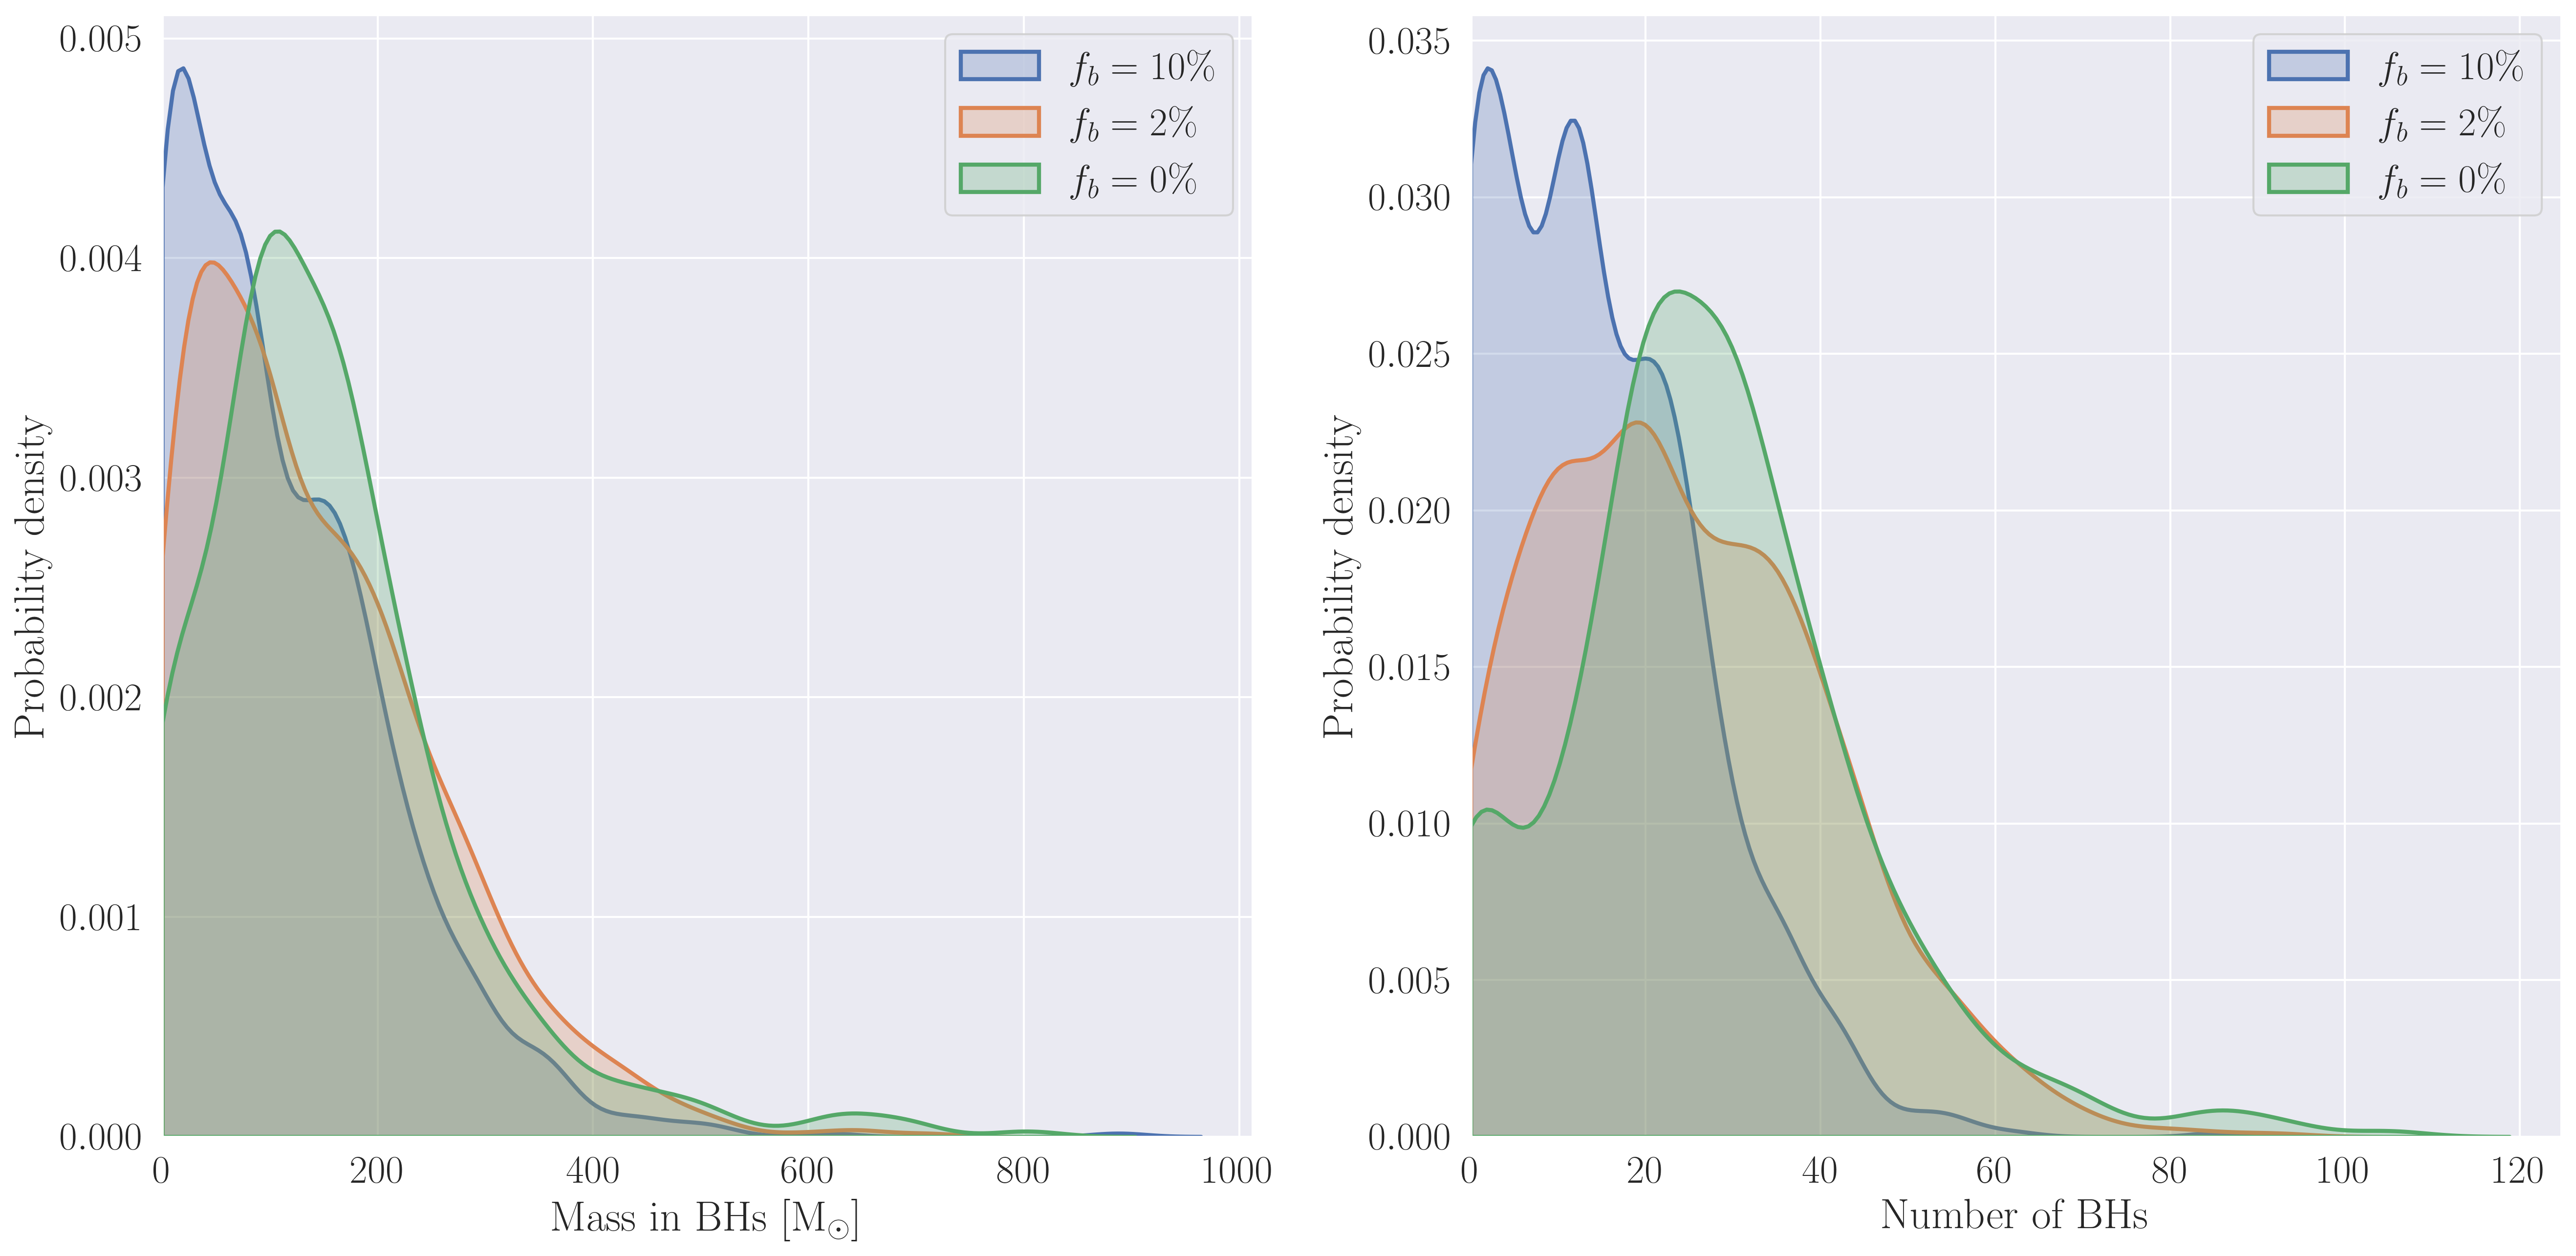
\includegraphics[width=\textwidth]{figures/BH_KDEs.png}
	\caption{Distribution of mass and number of BHs in each set of models. Distributions are
	 represented by a Kernel Density Estimate of the discrete values for easier visual
	 comparison.}
	\label{fig:BH_KDEs}
\end{figure}

When we examine the density profiles for the models with a binary fraction of $10\%$ (see Figure
\ref{fig:highbin_model_densities}), we can see that the binary stars are indeed more centrally
concentrated than typical main-sequence stars as predicted and in the central regions, make up
almost all the main-sequence contribution, while they contribute more than the neutron stars at all
radii.

\ps{Figure here showing enclosed mass in black holes, enclosed mass in binaries+black holes to show
	how binaries make up for some BHs. This might be a bit tricky, but it is a good way to see
	the effect}


\begin{figure}
	\centering
	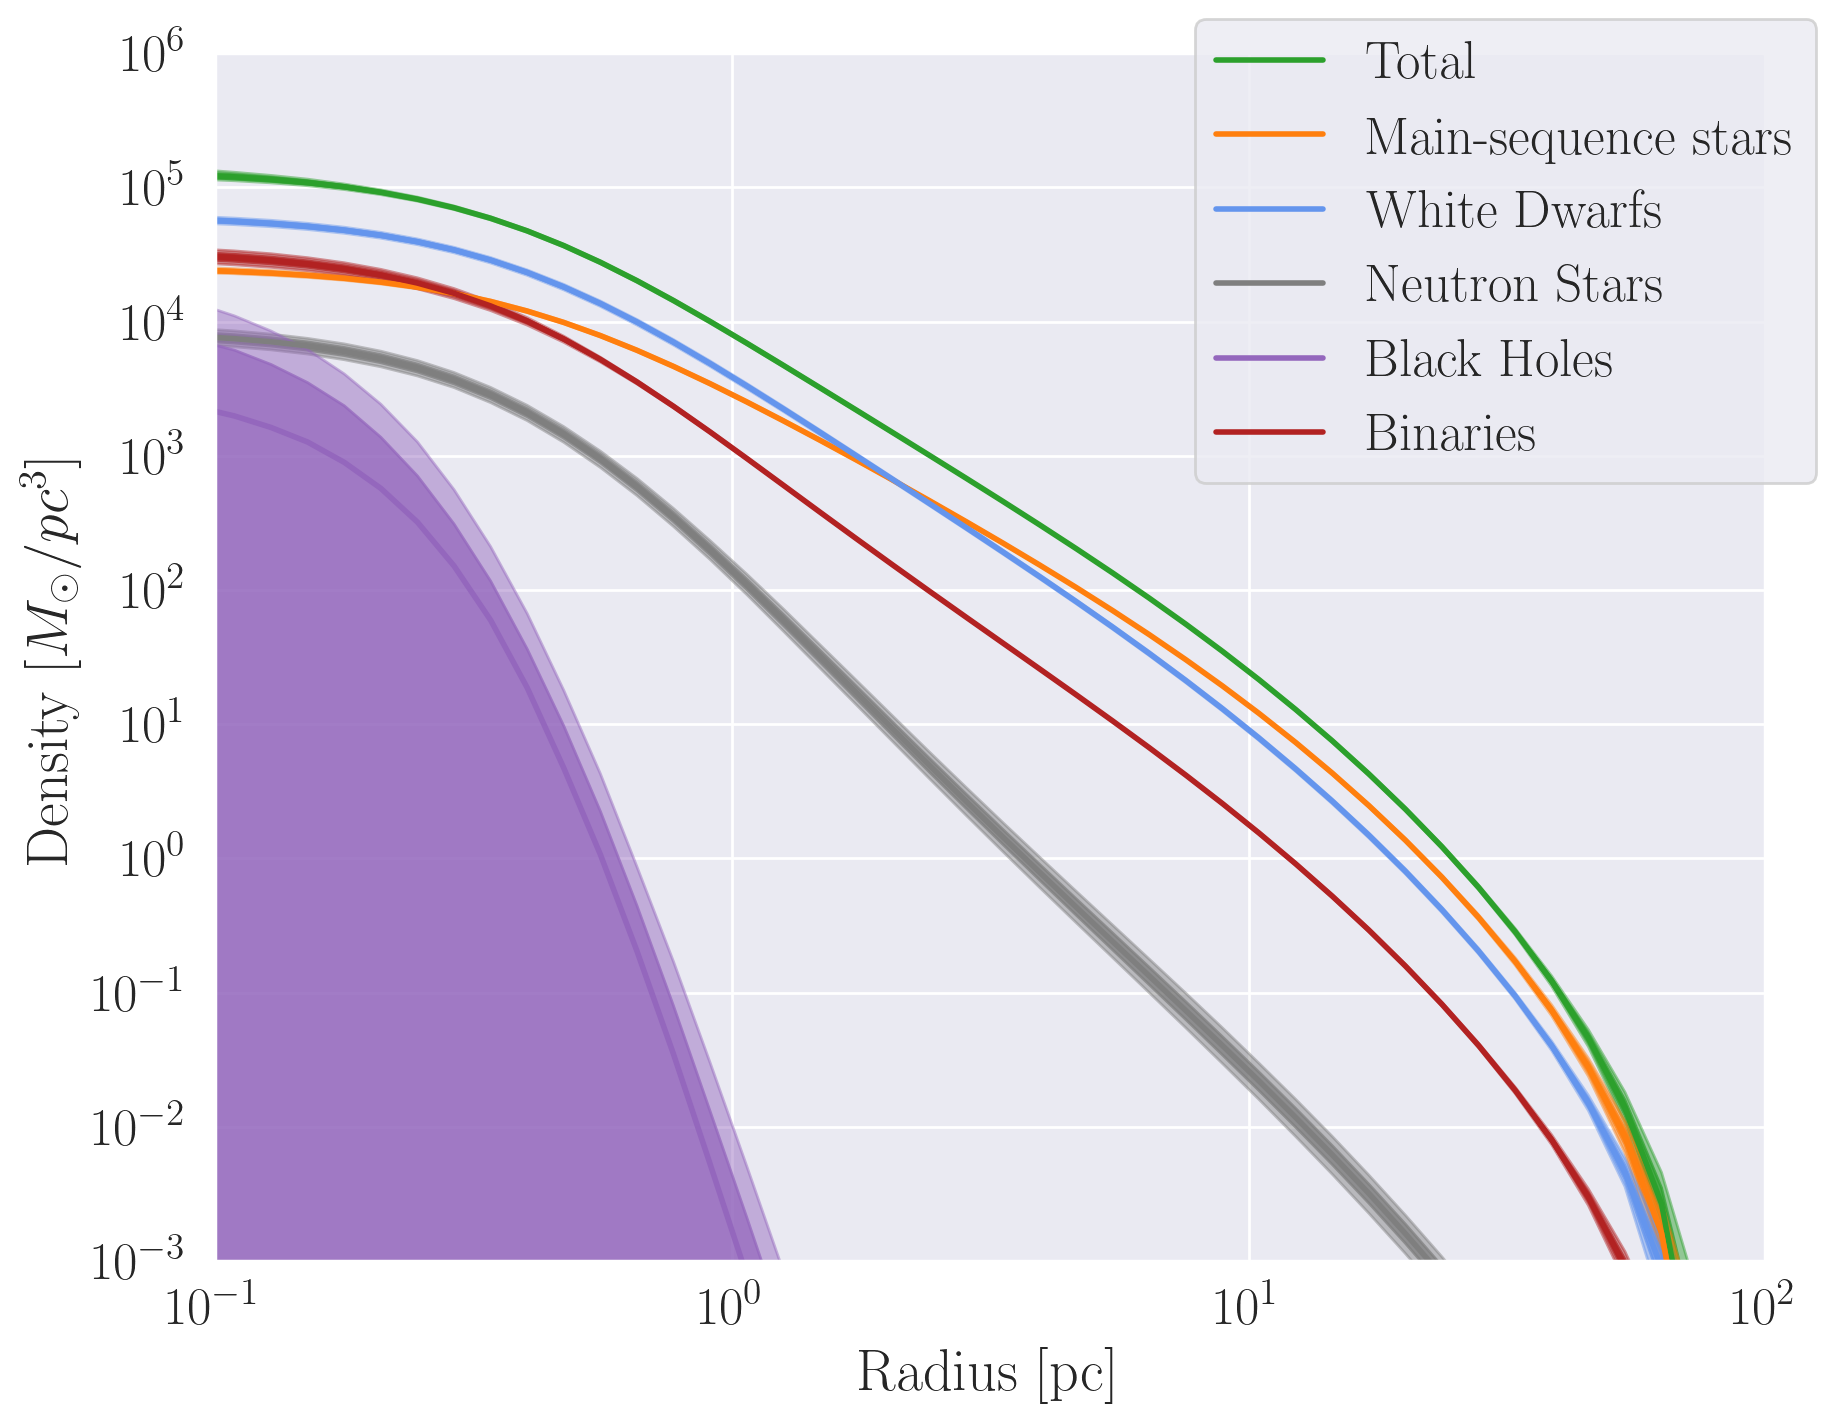
\includegraphics[width=0.8\textwidth]{figures/high_bin_model/density.png}
	\caption{Mass density profiles for the models with a binary fraction of $10\%$}
	\label{fig:highbin_model_densities}
\end{figure}



\subsection{Conclusion}


In summary, we have developed a method to include realistic binary populations in \code{LIMEPY}
models. We used this method to fit three sets of models to observations of the globular cluster
47\,Tuc, a set with no binaries, a set with a binary fraction of $2\%$, and a set with a binary
fraction of $10\%$. Despite their different binary fractions, all three sets of models were able to
satisfyingly reproduce all observables and recovered the same structural parameters for the models.
The three sets of models differed primarily in their recovered mass functions and black hole
content. As more binaries are added, few high-mass remnants are required to reproduce the kinematics
of the cluster. This results in a lowered $\alpha_3$ parameter and less mass in black holes.

The implications of this work depend on the binary fraction of the cluster in question. For 47\,Tuc,
our best estimates place the binary fraction at around $2\%$ this effect is likely negligible. If
however, future observations or models suggest that 47\,Tuc might be host to more binaries, then it
is important that future studies include their effects in their models if they wish to recover
accurate remnant populations. 


More generally, for clusters where we expect a high binary fraction like, for example, NGC\,3201,
binaries should certainly be included in any attempts to model the kinematic of the cluster,
especially if the goal is to constrain the population of heavy remnants within the cluster.



\subsection{Future Work}



In this work, we only considered binaries made up of two main sequence stars. In reality, binaries
can be formed from any cluster members and binaries where one or both components are heavy-remnants
would have an even larger effect on the kinematics of the cluster then main-sequence binaries. The
reason we did not consider this class of binaries in this project is because we have essentially no
constraints on what these populations might look like. The usual photometric methods cannot be used
because there is at most one main-sequence star and radial velocity search will only uncover them if
the binary contains a main-sequence star. It's possible that in this case, we could turn to N-body
or Monte Carlo models to constrain the present-day remnant binary populations, but the binary
populations in these models are likely to be highly dependent on the primordial binary population
and initial conditions of the models.

In the future it would be a nice application of this method to examine a cluster like NGC\,3201
where we know there is likely to be a fairly large binary population. This would allow us to place
fairly strong constraints on the black hole population in NGC\,3201 and also allow us to test the
relation between binary fraction and black hole content that we've demonstrated exists in 47\,Tuc. 